\chapter{Surface Event Pulse Shape Simulations}

\section{Surface Alphas}

\subsection{Properties of Alpha Interactions}
Alpha particles are composed of two protons and two neutrons tightly bound together. They are identical to ionized Helium ions and carry a charge of $+2$ e. The energy of alpha particles is correlated with the half-life of the parent isotope, such that the ones with the highest energies are from parent atoms with the shortest half-lives. Thus, the energies of alpha particles are normally between about $4$ and $6$ MeV. For a given material, the linear stopping power S is defined as $-\frac{dE}{dx}$. The energy loss of charged particles in a material is then given by the Bethe formula:

\begin{equation}\label{bethe_formula}
    -\frac{dE}{dx} = \frac{4\pi e^4z^2}{m_0\nu^2}NB
\end{equation}

such that

\begin{equation}\label{bethe_B}
    \text{B}=Z\left[ \text{ln}\frac{2m_0\nu^2}{I}-\text{ln}\right(1-\frac{\nu^2}{c^2}\left)-\frac{\nu^2}{c^2}\right]
\end{equation}

Here $\nu$ and $ze$ are the charges of the given particle, N and Z are
the number density and the atomic number of the absorber atoms, and  m$_0$ and e are the rest mass and charge of electron respectively. Parameter I represents the average excitation and ionization potential of the absorber and is normally determined experimentally. Eq. \ref{bethe_formula} suggests that the energy loss for non-relativistic particles is proportional to $1/\nu^2$, or the kinetic energy. This can be understood by noting that the smaller the velocity, the longer the particles spend in the vicinity of electrons of the material's atoms, and the higher the energy loss. Eq. \ref{bethe_formula} is proportional to z$^2$ for constant velocity. Thus heaver particles will have more energy loss for a given velocity. This results in alphas having a very low penetration depth, usually around $10$ micrometers.

Energy loss of alpha particles can be best understood by plotting specific energy loss along the track. The plot known as the Bragg curve is shown in Fig. \ref{bragg_curve_fig}. During most of the track, the energy loss increases roughly as 1/E as predicted by Eq.\ref{bethe_formula}. As the particles slow down, electron pickup reduces the charge and the curve falls off. A result of these curves is that alpha deposits a large amount of energy in a very localized area. For Germanium, the penetration depth of alpha particles is about $17.6$ - $20.0$ microns. The n+ electrode and p+ electrode in LEGEND detectors are too thick for alphas to penetrate and deposit much energy. However, the passivated surface experiences complex surface effects which are described next.

\begin{figure}
\centering
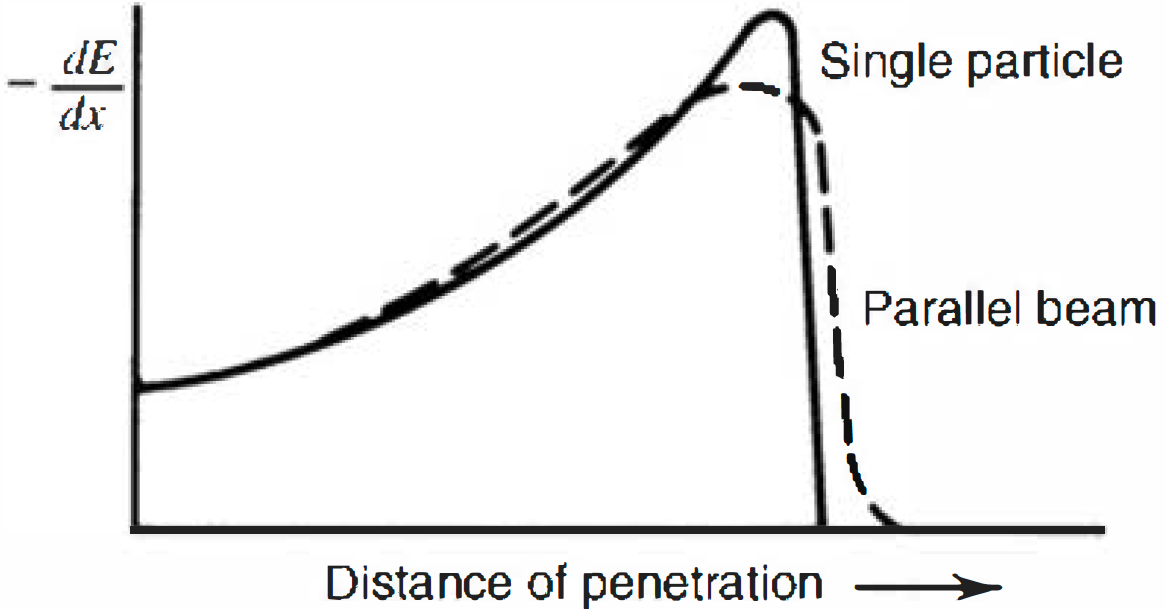
\includegraphics[width=0.5\linewidth]{ch3/figs/bragg_curve.png}
\caption{The specific energy loss in a material for an alpha particle with several MeV initial energy. Plots are shown for a single alpha particle track and for the average behavior of a parallel beam of alpha particles \cite{knoll_2010}}. 
\label{bragg_curve_fig}
\end{figure}

% \subsection{The DCR effects}

% The behavior of alphas on the passivated is not well understood. Charge trapping and subsequent slow rerelease have been observed on the surface. These effects might be different for different detector types. For PPC detectors the electric field near the passivated surface can lead to the charges drifting along the surface. It has been shown using Monte Carlo simulations of hole drift in HPGe crystals that surface charges drift 10 to 100 times slower than bulk charges. A combination of slow drift, charge trapping, and re-release results in a slow component in the alpha signal, as shown in Fig. \ref{fig:dcr_waveform} 

% \begin{figure}
% \centering
%   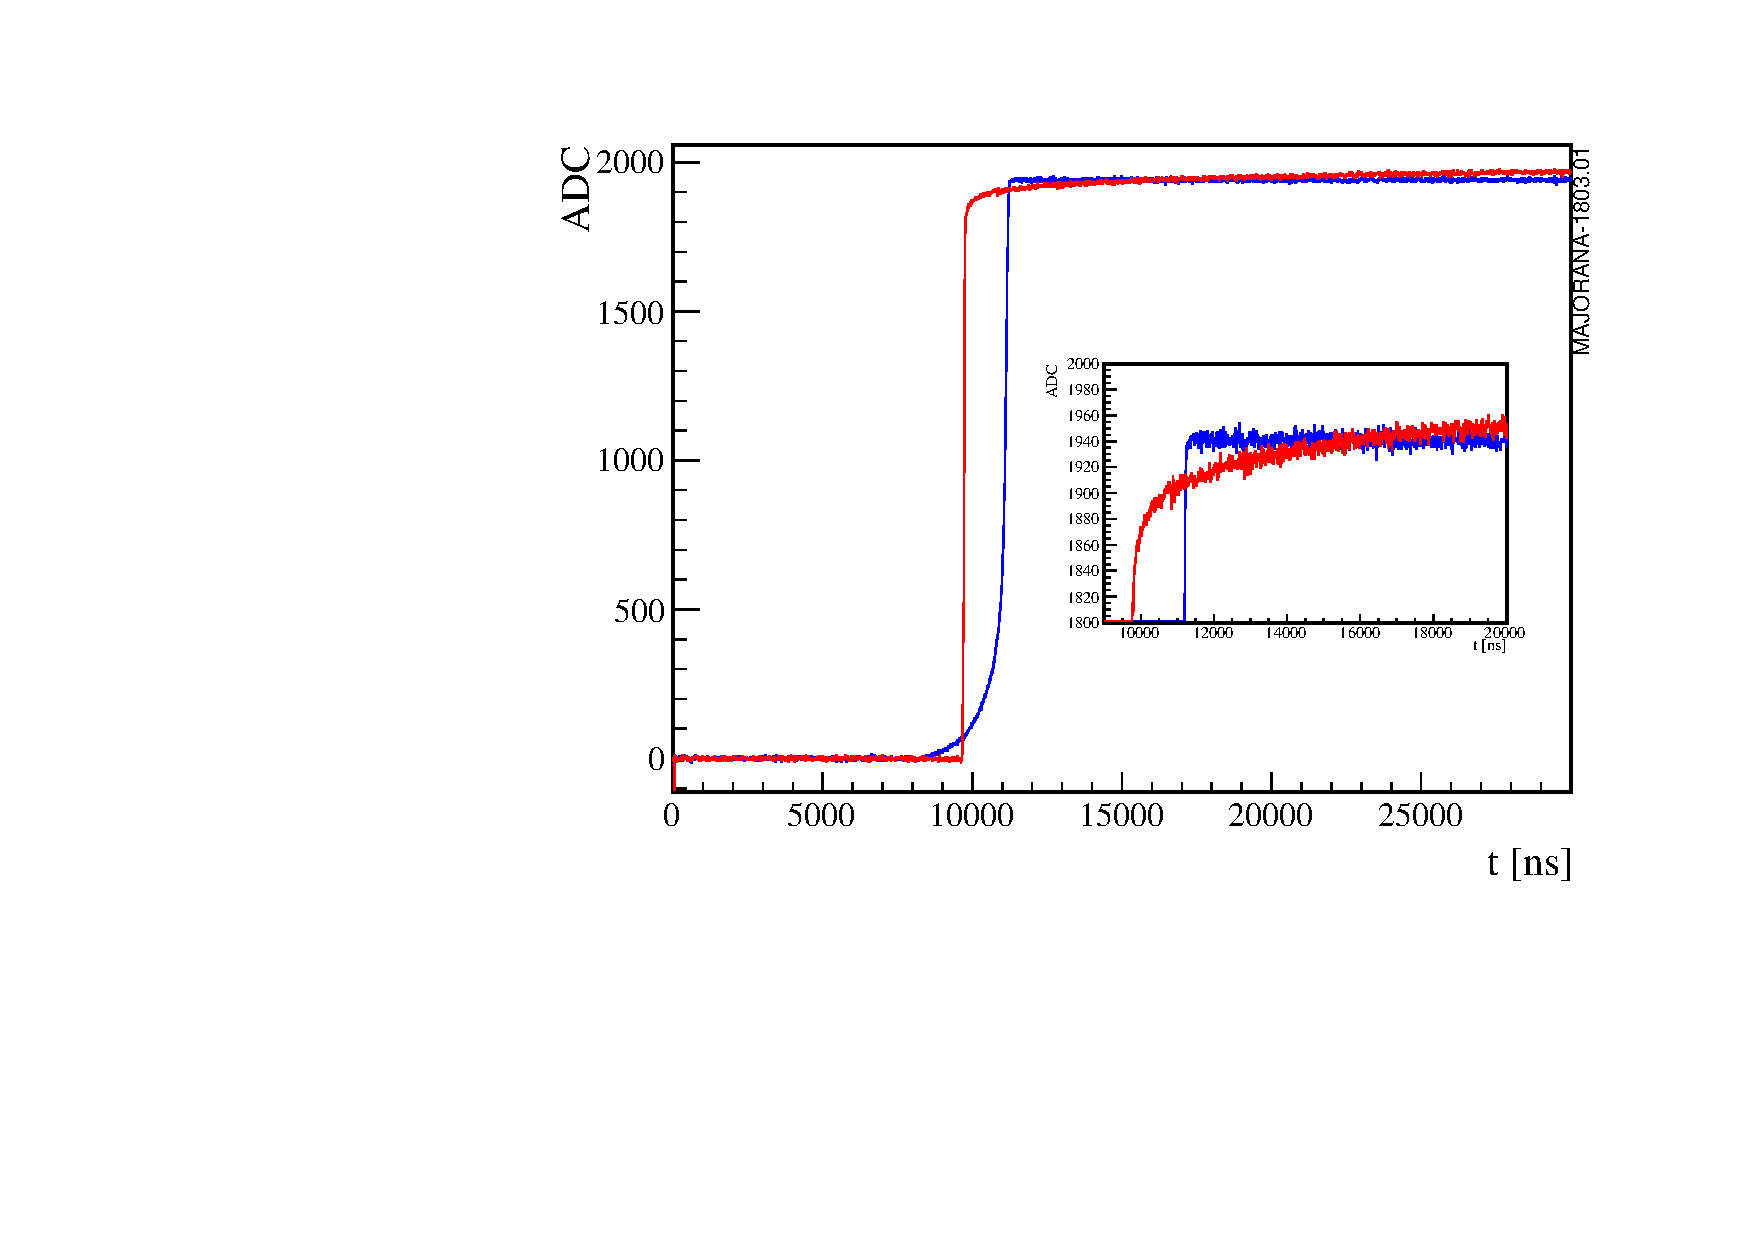
\includegraphics[width=0.6\linewidth]{ch3/figs/dcr_waveform.pdf}
%   \caption{An alpha waveform (red) compared to a bulk waveform (blue) in MJD PPC detector. The slow components result in a distinct tail with a smaller slope, as shown by the highlight area in the box.}
% \label{fig:dcr_waveform}
%   \end{figure}
  

%  \begin{figure}[htb]
% \centering
%   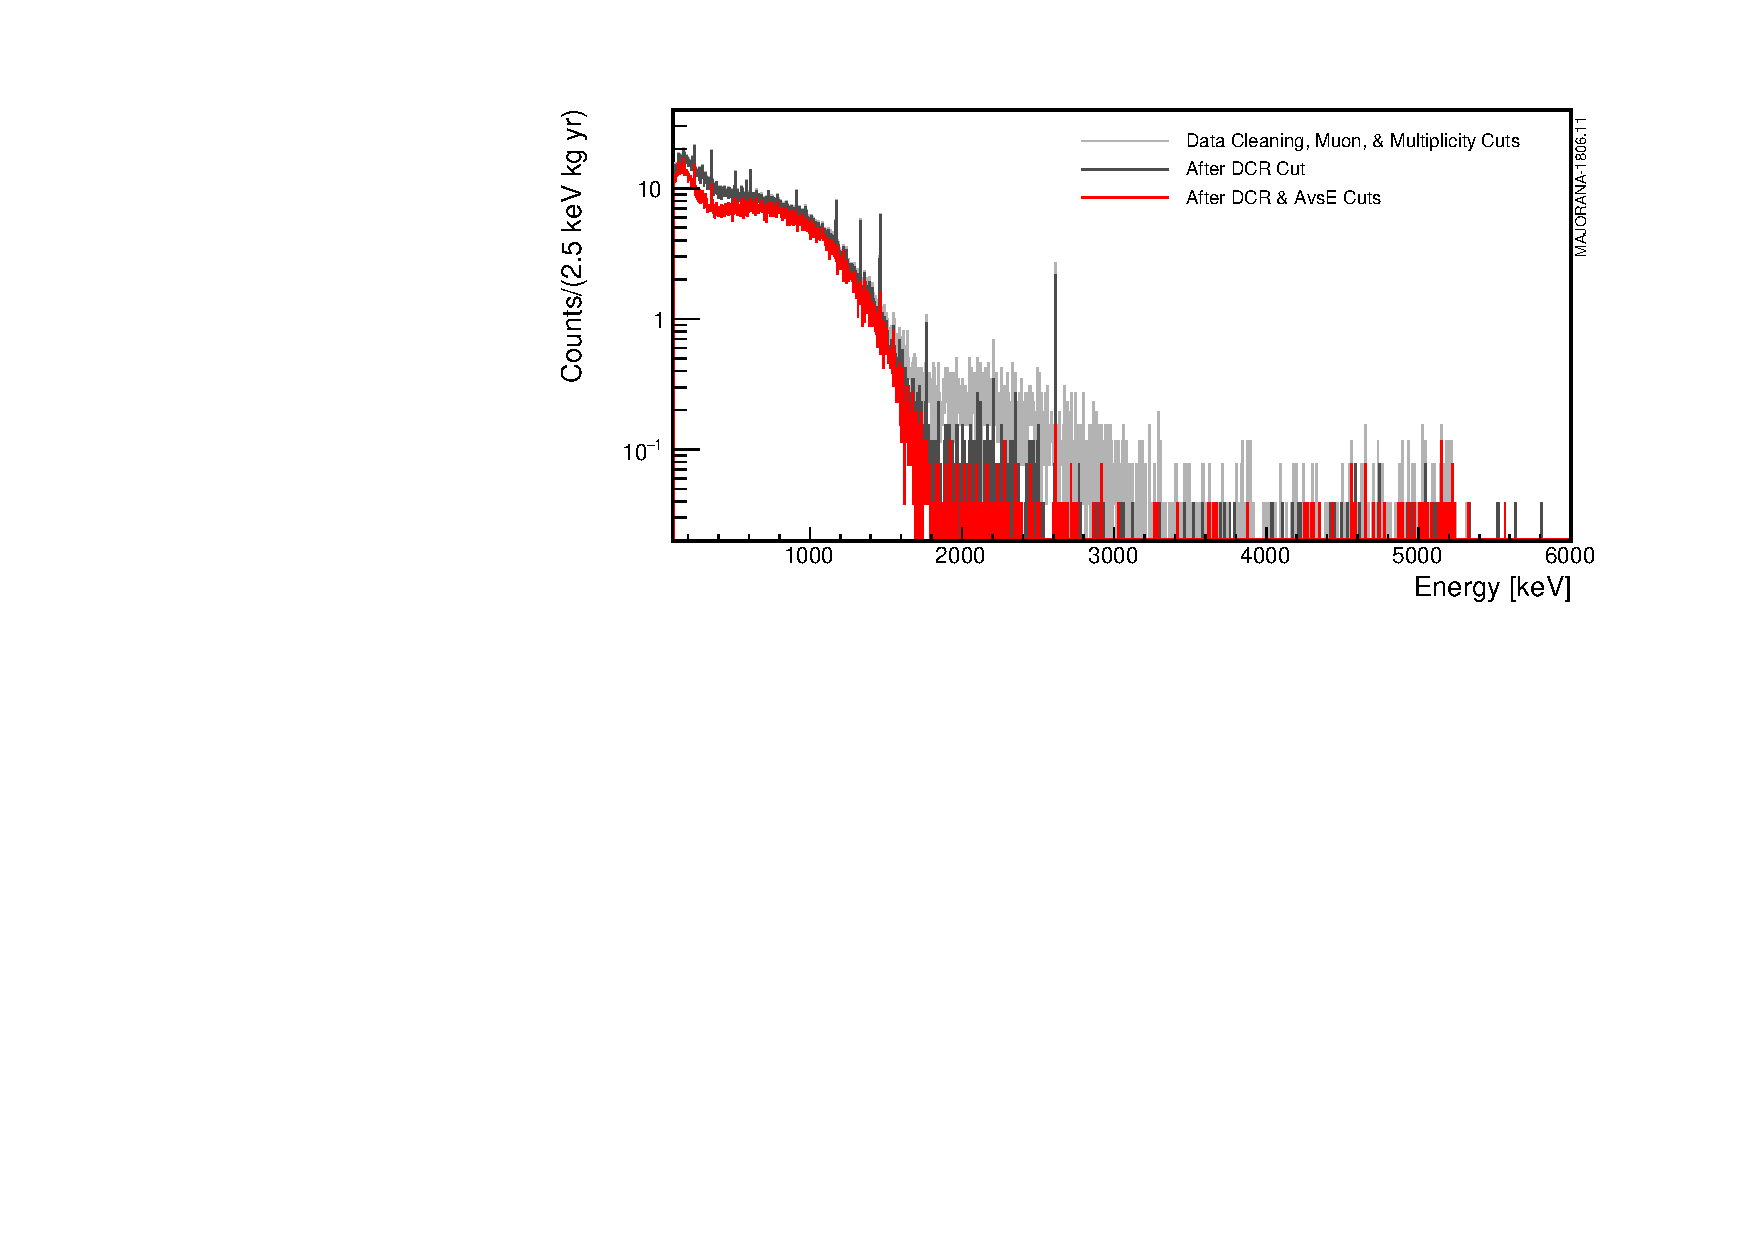
\includegraphics[width=0.8\linewidth]{ch3/figs/mjd_alpha.pdf}
% 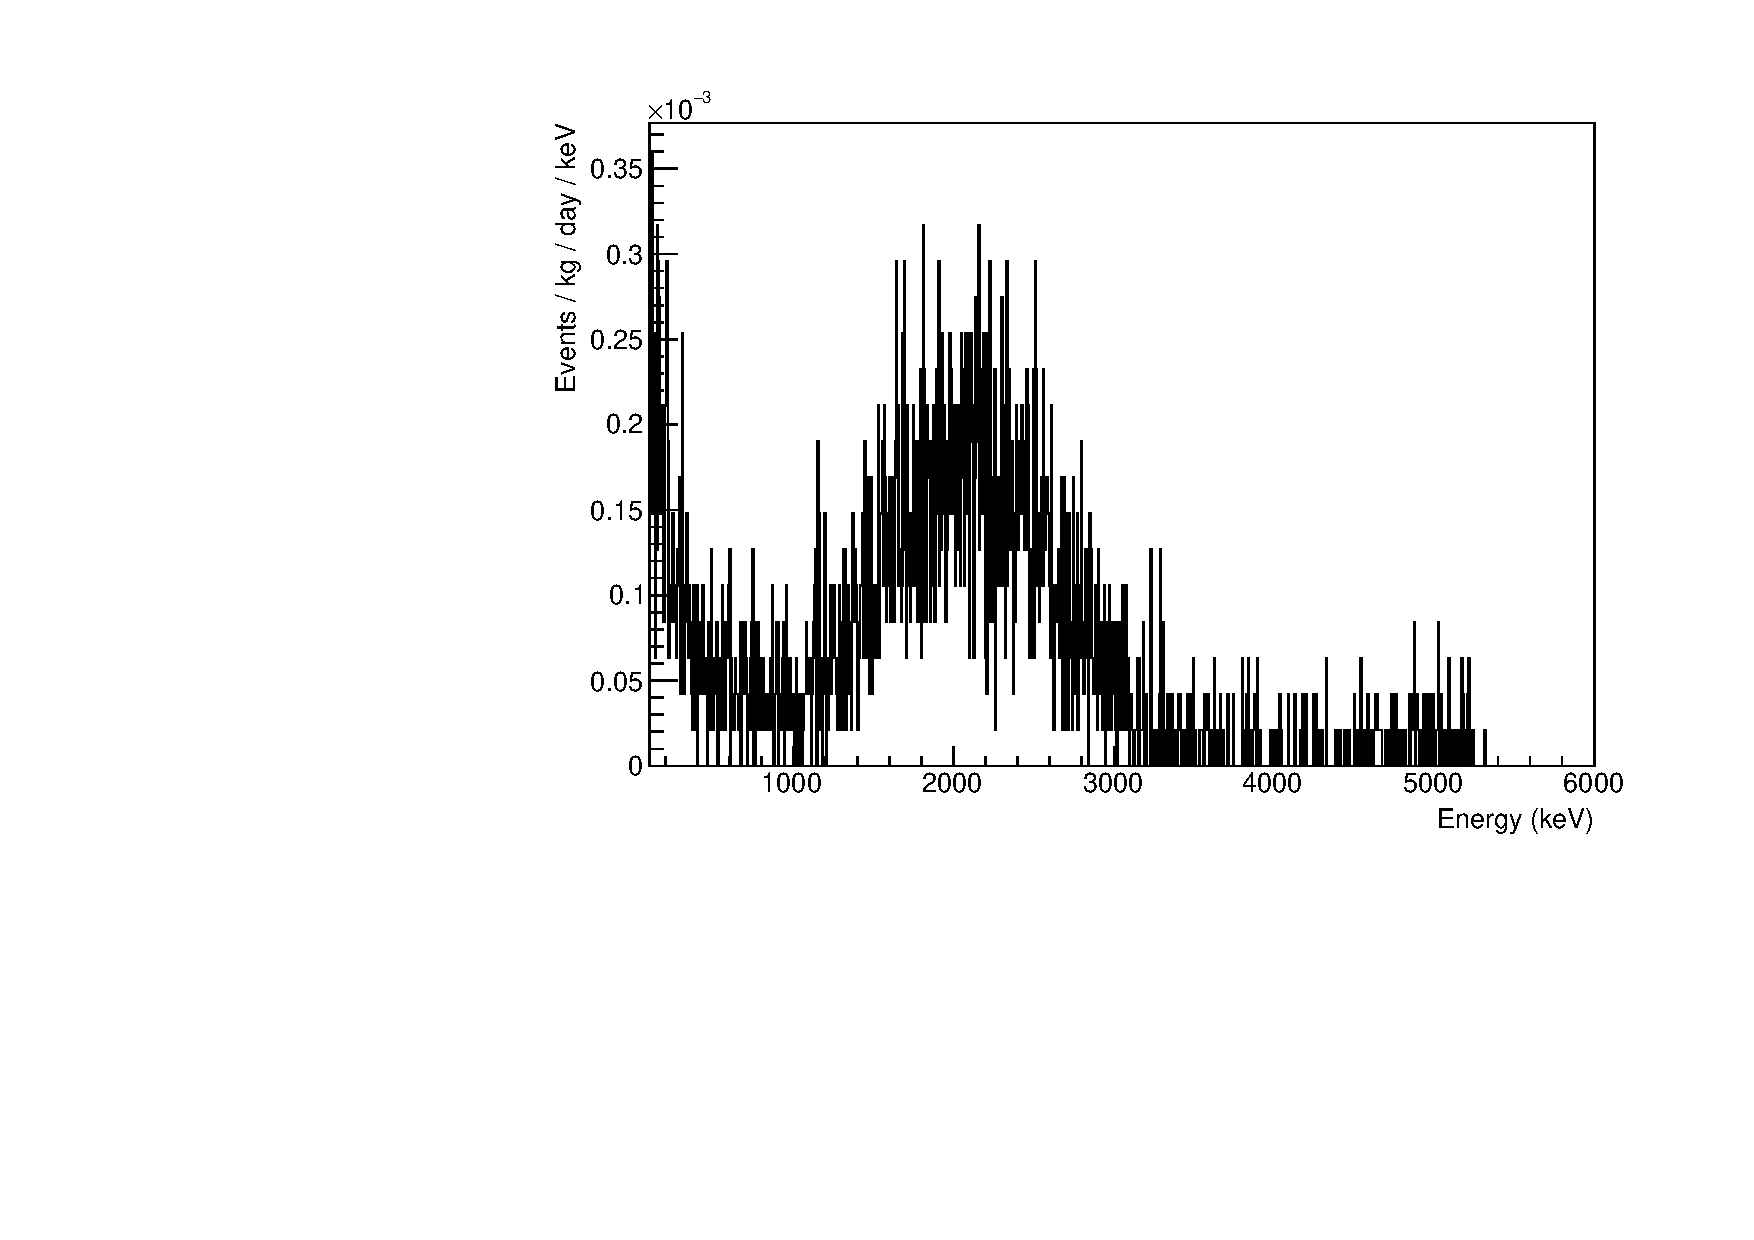
\includegraphics[width=0.5\linewidth]{ch3/figs/MJD_alpha_spec.pdf}
%   \caption{Top: MJD energy spectrum. The light grey line are the events after data cleaning, Muon and multiplicity cuts, and the grey lines are after DCR cuts that remove alpha events. Bottom: The alpha energy spectrum in MJD calculated using the events before and after the DCR cut.}
% \label{fig:mjd_alpha}
%   \end{figure}

\section{Challenges in modeling surface events}
An alpha particle deposits energy of about $4$ - $6$ MeV with a penetration depth of about $17.6$ - $20.0$ micron \cite{knoll_2010}. This excites a lot of charge carriers and produces a dense charge cloud. In such cases, effects such as diffusion of the charges and self-repulsion among charges become significant. Self-repulsion could also push the charge onto the passivated surface, leading to a slower drift and longer collection time for these charges. This slow drift is thought to be due to a combination of charge trapping and re-release near the passivated surface, and slower drift speeds due to surface properties \cite{MULLOWNEY201233}. The passivated surface could also carry a static charge, which could affect the charge collection. In experimental data, these effects manifest as an energy-degraded alpha waveform with a slow rising tail, as shown in Fig. \ref{fig:dcr_waveform}.

  \begin{figure}[!htb]
\centering
  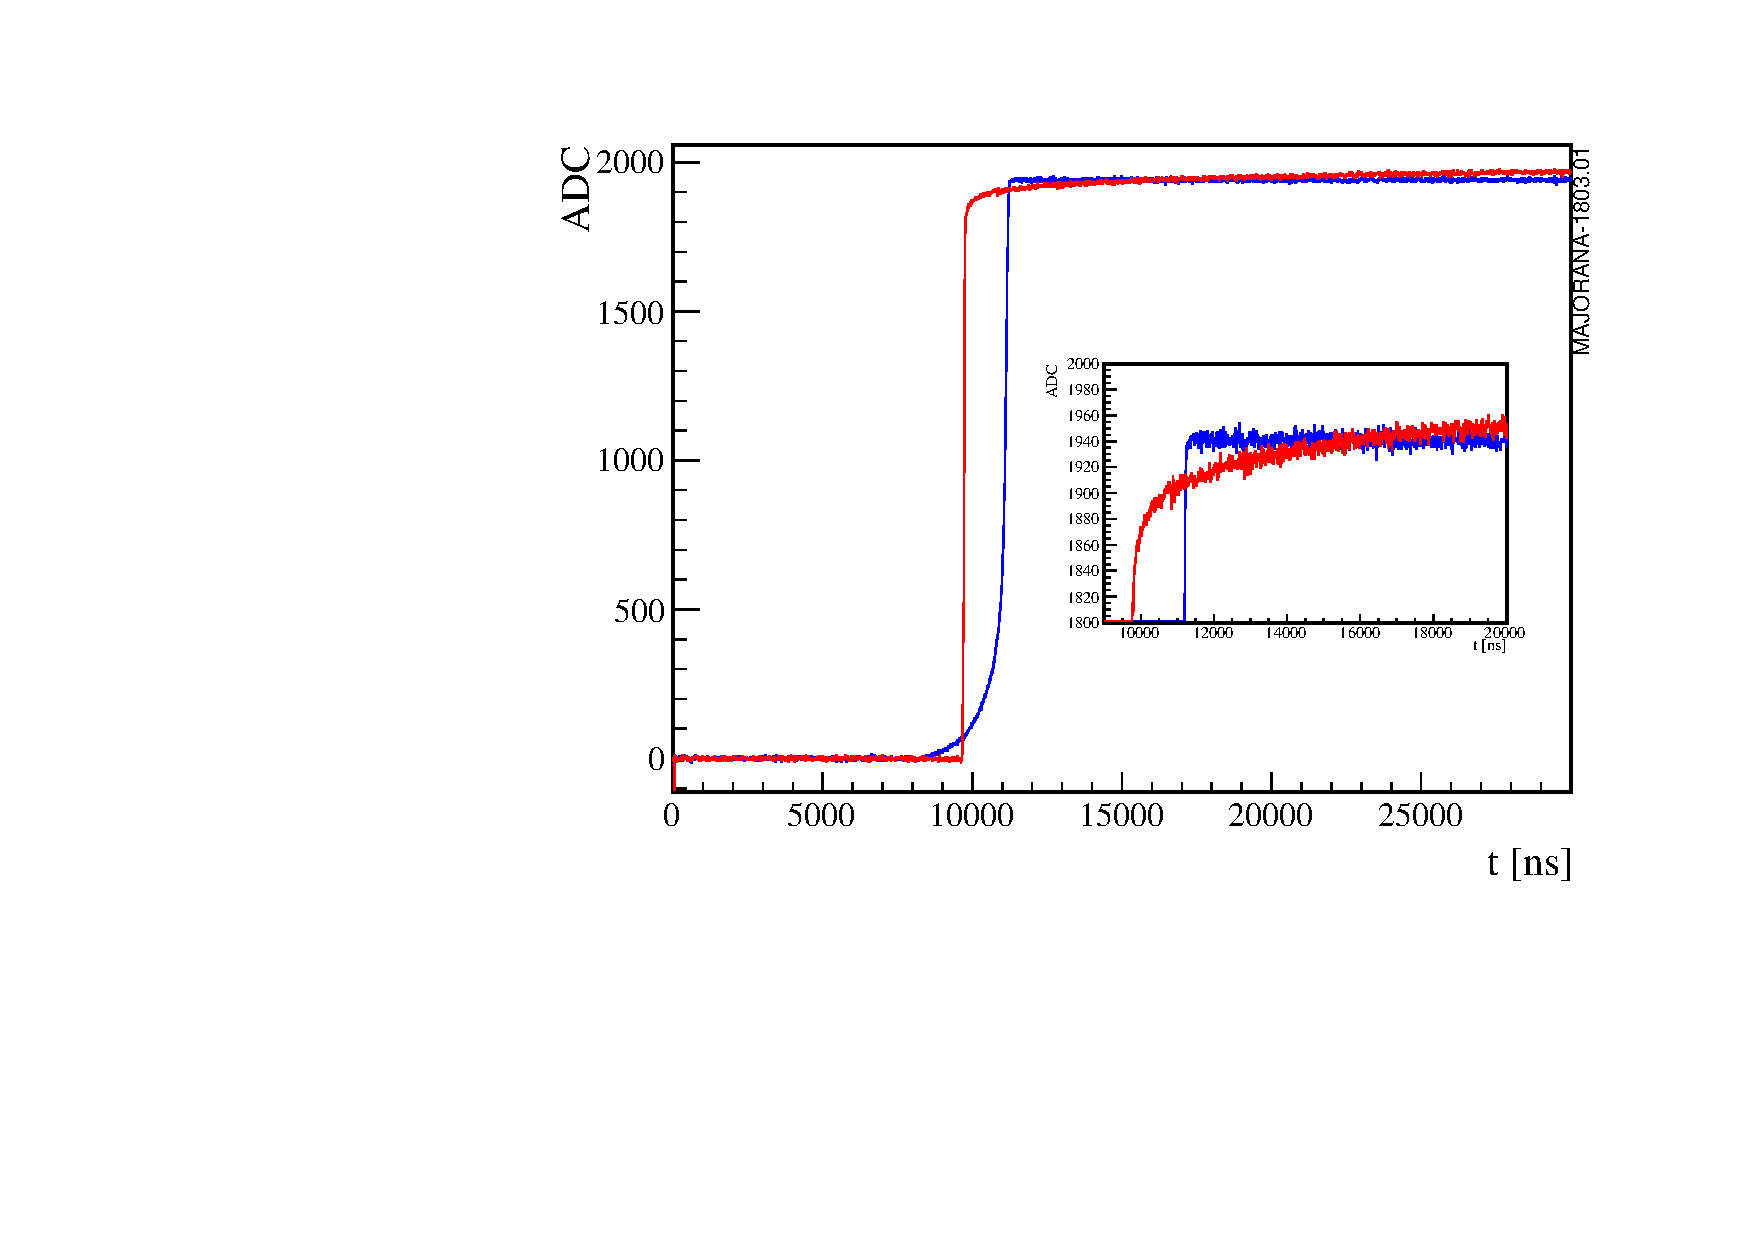
\includegraphics[width=0.8\linewidth]{ch3/figs/dcr_waveform.pdf}
 \caption{An alpha waveform (red) compared to a bulk waveform (blue) in the MJD PPC detector. The DCR effect results in a distinct tail with a smaller slope, as shown by the highlight area in the box.\cite{tube_paper}}
\label{fig:dcr_waveform}
  \end{figure}

 This DCR effect results in energy degradation in the alpha signal. Even though alphas are normally deposited with $5$ MeV energy, the degraded energy could lead alpha events potentially appearing in the ROI. Fig. \ref{ch3_fig_L200_surface_background} shows the LEGEND physics spectrum. Muon and multiplicity remove background such as muons and gamma rays, and the events left are primarily surface events shown in grey. This spread-out spectrum is due to the DCR effect. As shown in green, PSD cuts are highly effective in removing them, but the unknown efficiency of those cuts introduces uncertainty in the background model. 

  \begin{figure}[!htb]
\centering
  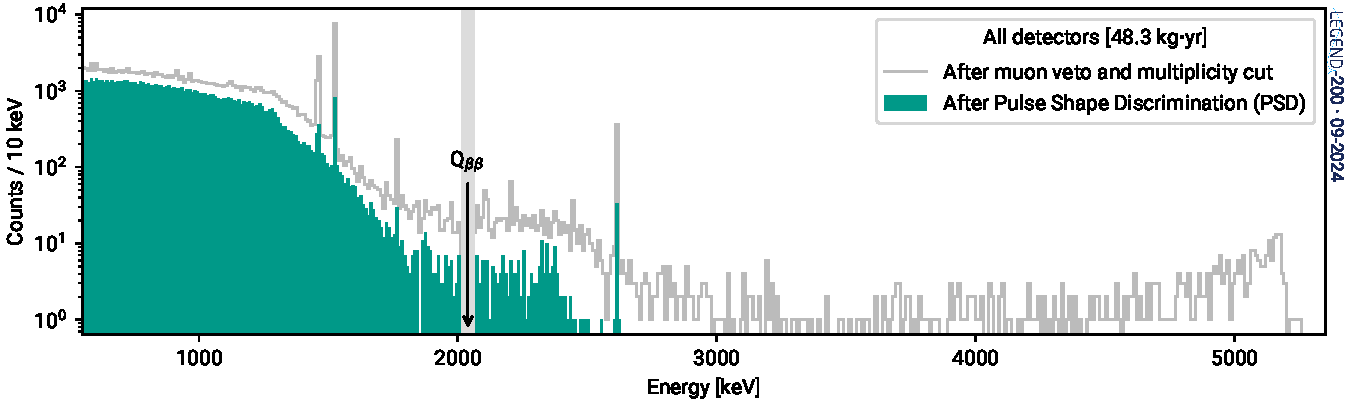
\includegraphics[width=0.99\linewidth]{ch2/figs/l200-phy-spectrum-psd.pdf}
  \caption{{\Ltwo} physics spectrum. The events above 3000 kev after the muon and multiplicity cut are primarily alphas. These events can be effectively remove using PSD cuts as show in green. Credit: Luigi Pertoldi}
\label{ch3_fig_L200_surface_background}
  \end{figure}

\section{Surface Charge Effect}
Due to various factors such as manufacturing, experimental conditions, and transportation, the HPGe detectors can develop charge on the passivated surface. This could impact charge collection for surface events. Fig. \ref{ch3_fig_surface_field_sc0} shows how the presence of surface charge influences the electric field close to the passivated surface. When there is no surface charge (top), the field lines are parallel to the surface. Presence of negative surface charge (middle) attract the field lines towards the surface. Positive surface charge (bottom) repels the field lines from the surface. Negative surface charge can pull the holes to the surface where they can drift slowly. Similarly, positive surface charges can pull the electrons to the surface.

% \clearpage
\begin{figure} %[!htb]
\centering
%[trim={left bottom right top},clip]
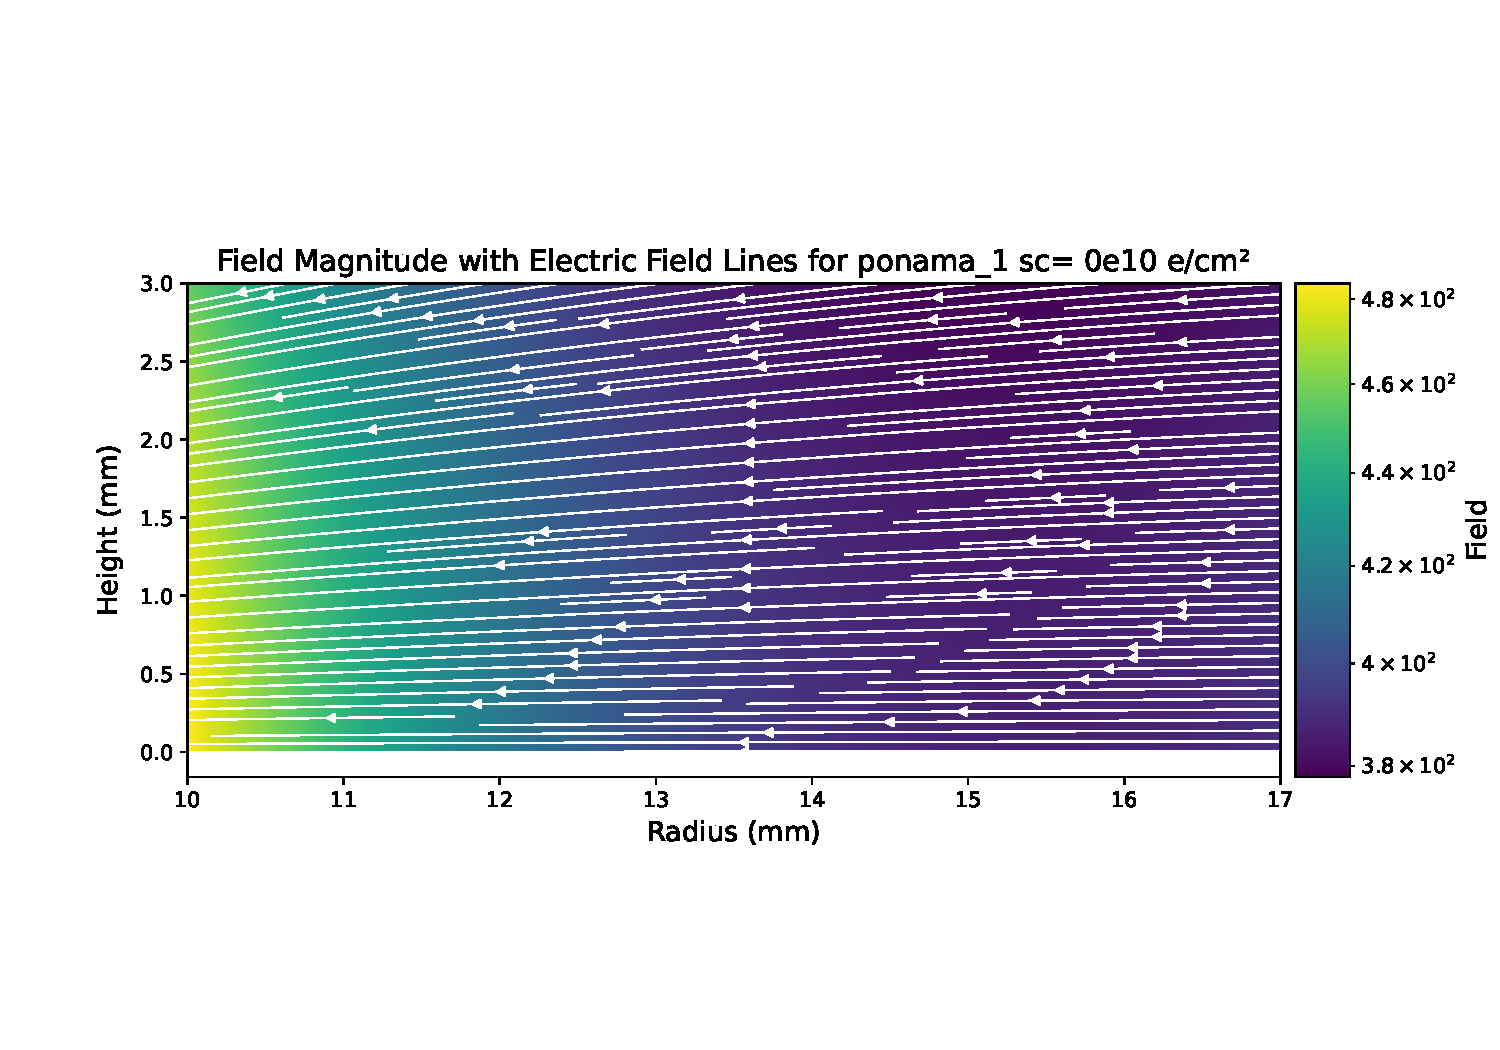
\includegraphics[trim={1cm 3.5cm 0.5cm 4.0cm},clip,width=0.99\linewidth]{ch3/figs/elect_field_lines_surface_ponama_1_sc_0.pdf}
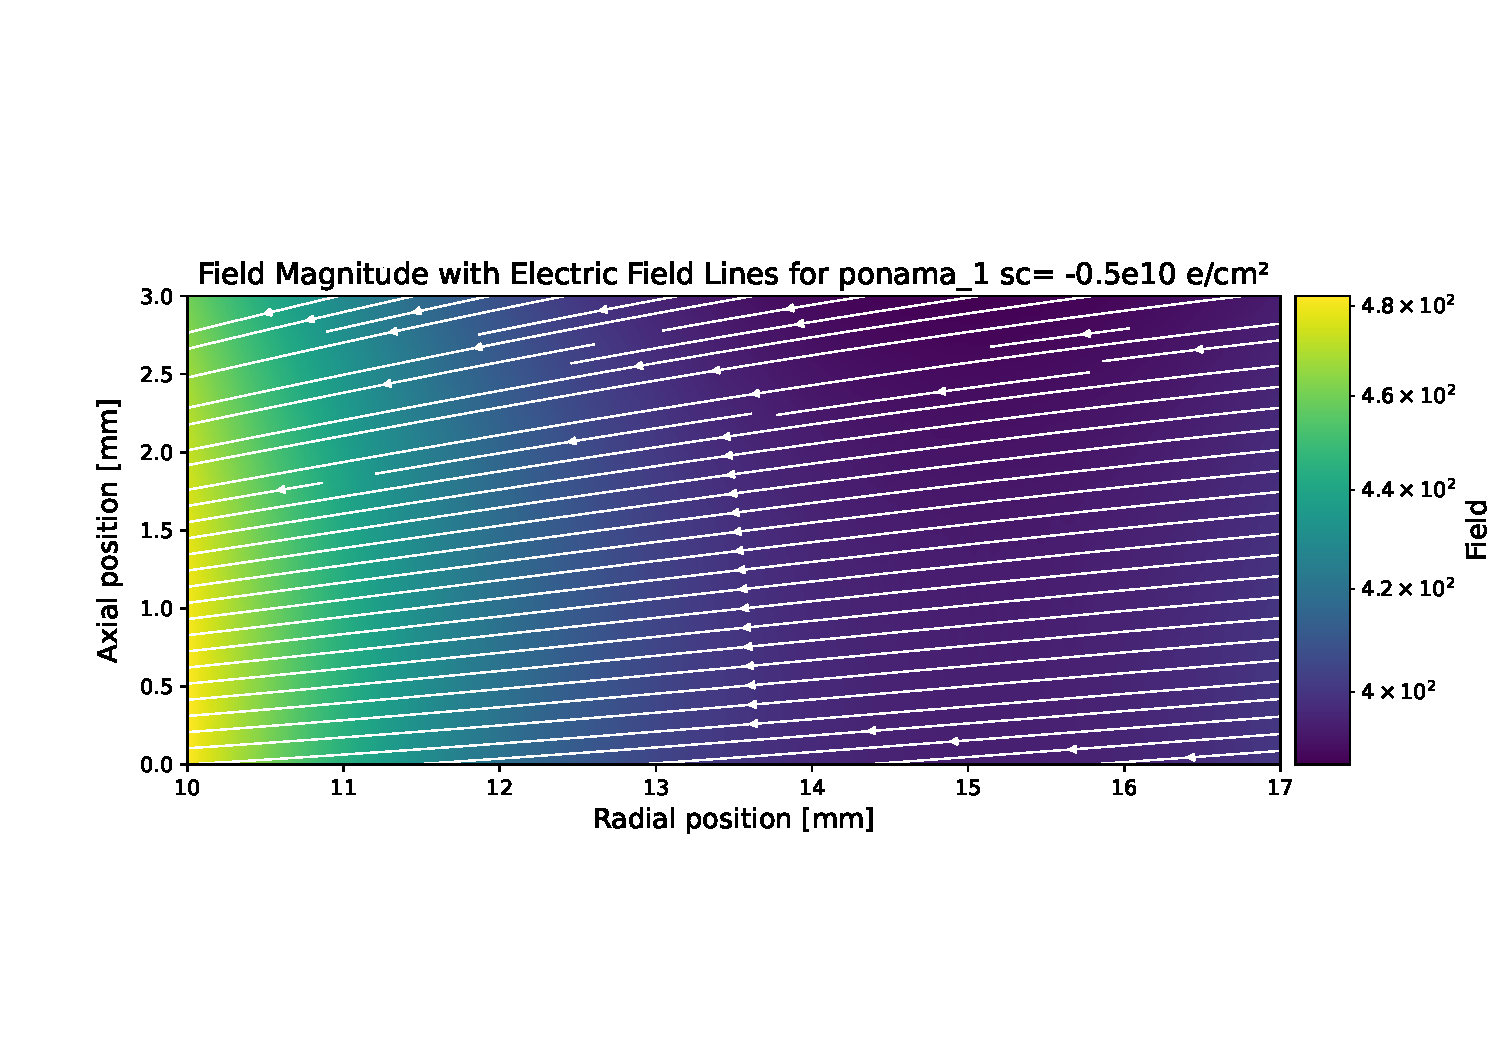
\includegraphics[trim={1cm 3.5cm 0.5cm 4.0cm},clip,width=0.99\linewidth]{ch3/figs/elect_field_lines_surface_ponama_1_sc_-0.5.pdf}
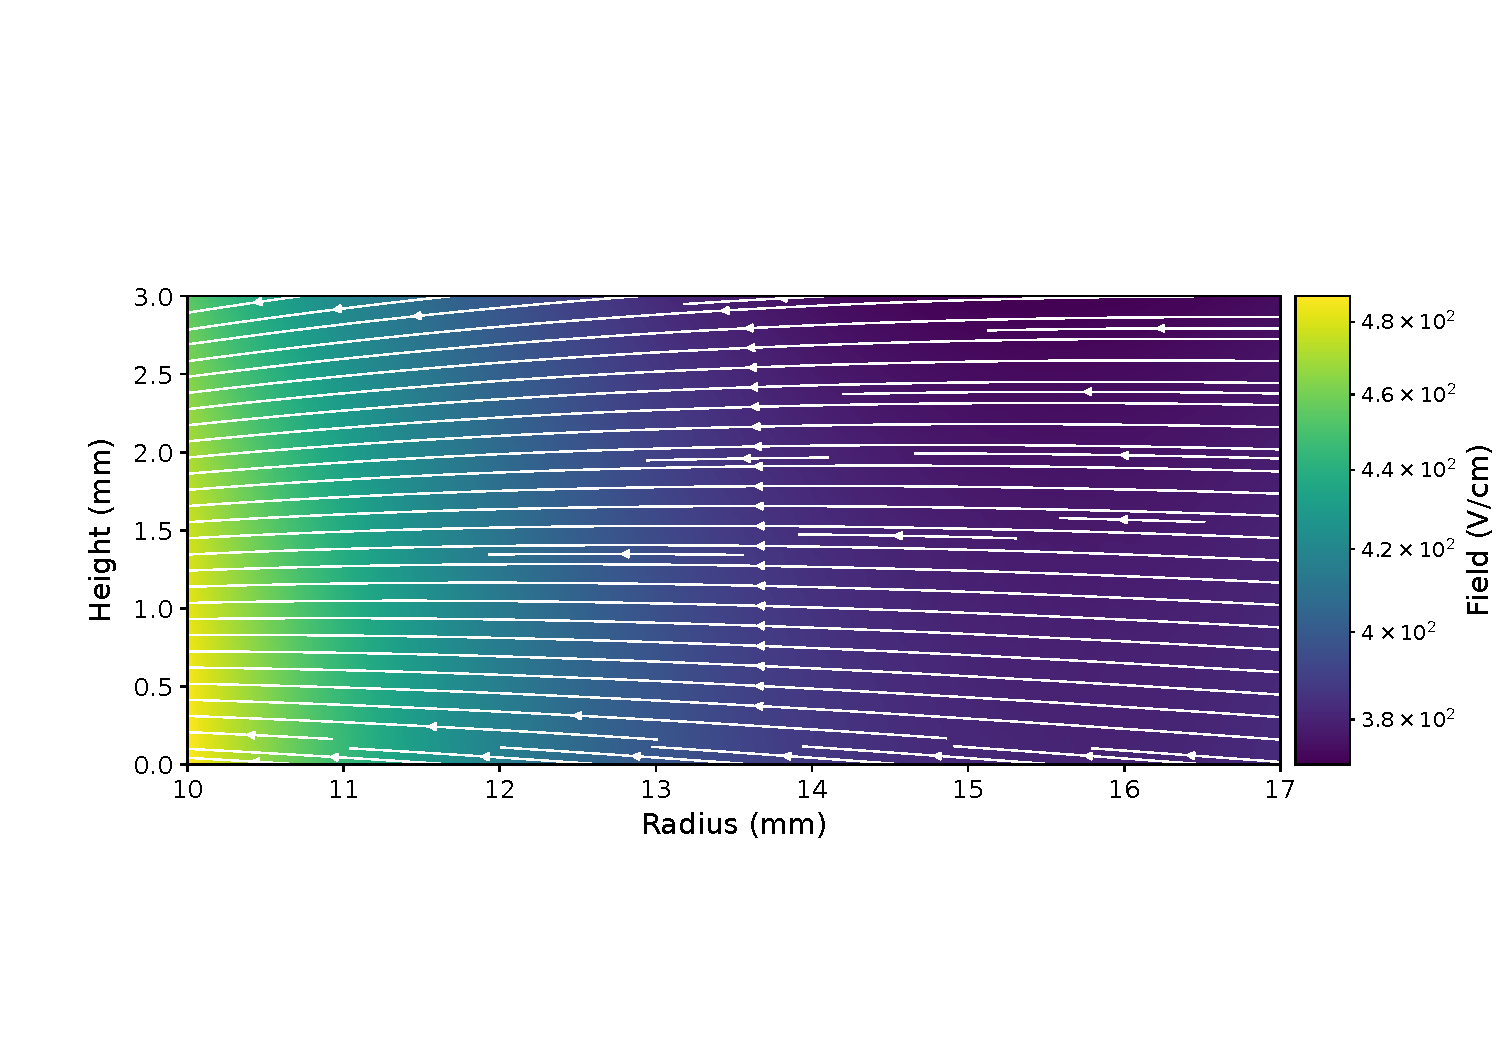
\includegraphics[trim={1cm 3.5cm 0.5cm 4.0cm},clip,width=0.99\linewidth]{ch3/figs/elect_field_lines_surface_ponama_1_sc_0.5.pdf}
\caption{Electric field magnitude and lines for the passivated surface of a PPC detector with different surface charges.}
\label{ch3_fig_surface_field_sc0}
\end{figure}


Surface charges can also change the overall electric field of the detector and impact the depletion voltage for the detector. Fig. \ref{ch3_fig_deplection_sc} shows how the depletion voltage for a LEGEND PPC detector changes with surface charge. Typically detector's operational voltage is higher than the depletion voltage, but if the surface charges is not properly account for, a detector could be left undepleted in the experiment.

\begin{figure}[!htb]
\centering
  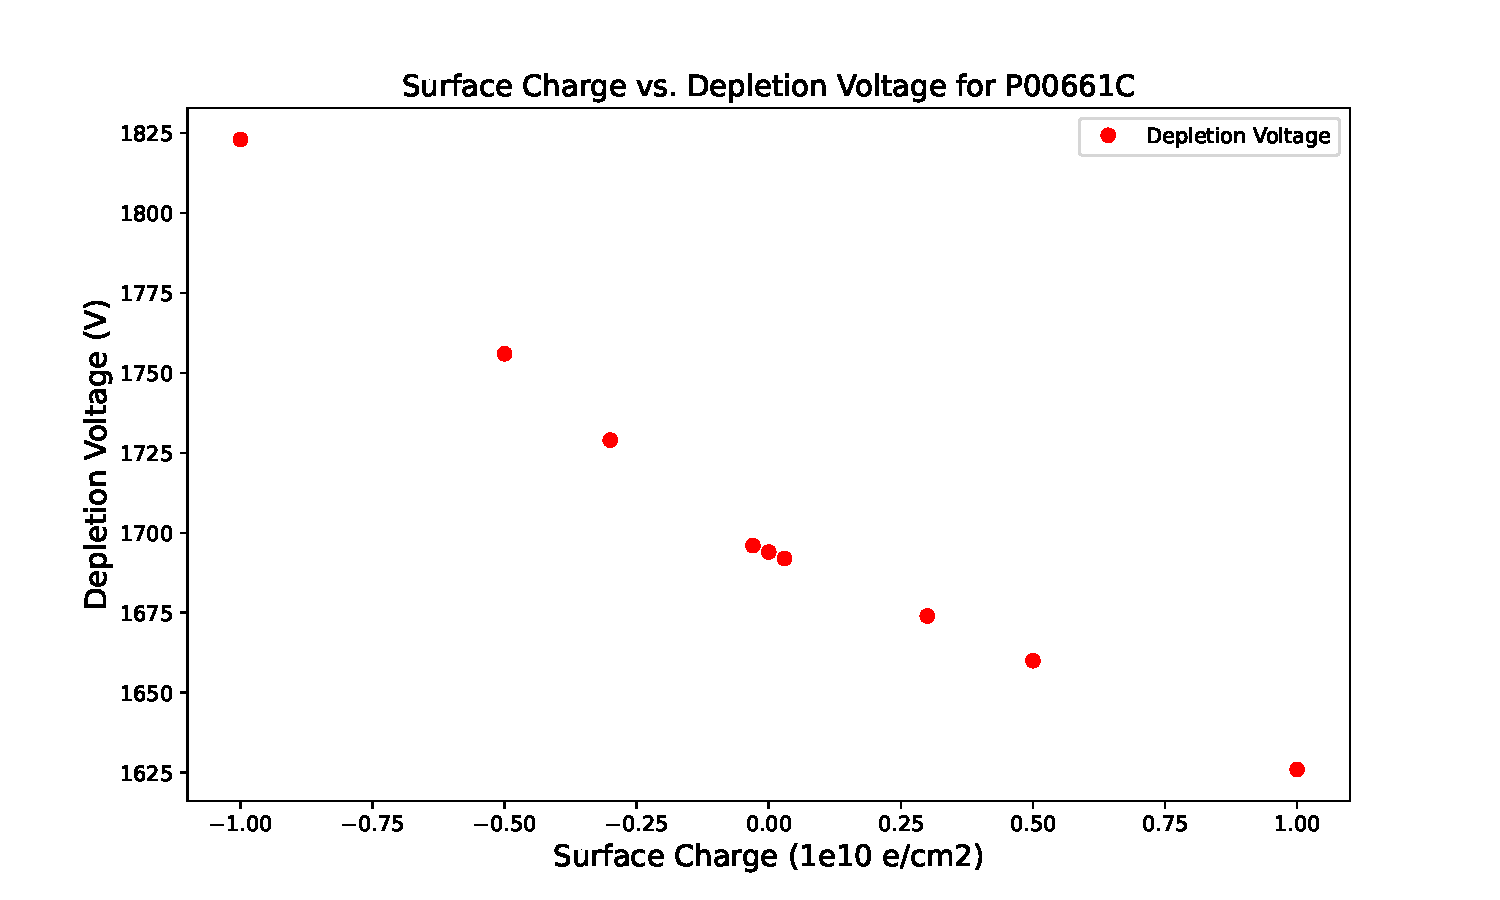
\includegraphics[width=0.99\linewidth]{ch3/figs/deplep_sc.pdf}
 \caption{Effect of surface charge on depletion voltage for LEGEND PPC detector. Depletion voltages calcuated using \texttt{siggen} software.}
\label{ch3_fig_deplection_sc}
  \end{figure}

Pulse-shaped simulations can help accurately these effects and build a background model for surface events. A simulation to model surface events should allow for a nonspherical charge cloud while incorporating surface drift, diffusion, and self-repulsion. They should also properly account for surface charge effects. We look at the current pulse shape simulations framework used by LEGEND.

\section{Pulse shape simulations till now}

Signal formation in Germanium is well understood via the Shockley-Ramo theorem. This enables building accurate simulations that can model the waveforms. Simulations within the LEGEND collaboration include \texttt{siggen} and \texttt{SSD} simulations. 

\texttt{siggen} is a C-based program initially developed by David Radford at Oak Ridge National Lab for MJD pulse shape simulations \cite{siggen_paper}. It consists of two components: \texttt{fieldgen} and \texttt{siggen}. \texttt{fieldgen} is used to calculate the electric potential and weighting potential of point-contact detectors in two-dimensional cylindrical coordinates. The \texttt{siggen} part uses the weighing potential calculated from \texttt{fieldgen} to generate a signal. The simulations can calculate the depletion voltage, the volume of the depletion region, and the capacitance of the detector. Diffusion in \texttt{siggen} is approximated using a Gaussian convolution, and there is no mechanism to account for the self-repulsion of charges as \texttt{siggen} uses point charges to represent the entire charge cloud.

% A simulated event in \texttt{siggen} is shown in Fig. \ref{fig:\texttt{siggen}_1d}.

% \begin{figure}
% \centering
% 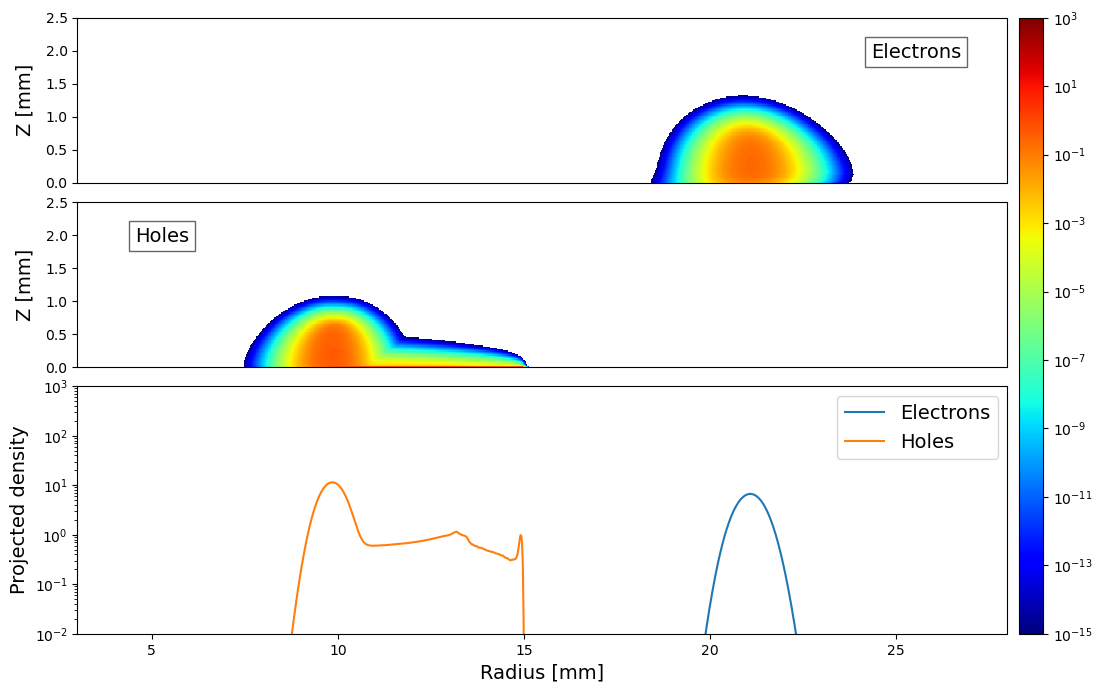
\includegraphics[width=0.49\linewidth]{ch3/figs/drift_path.png}
% 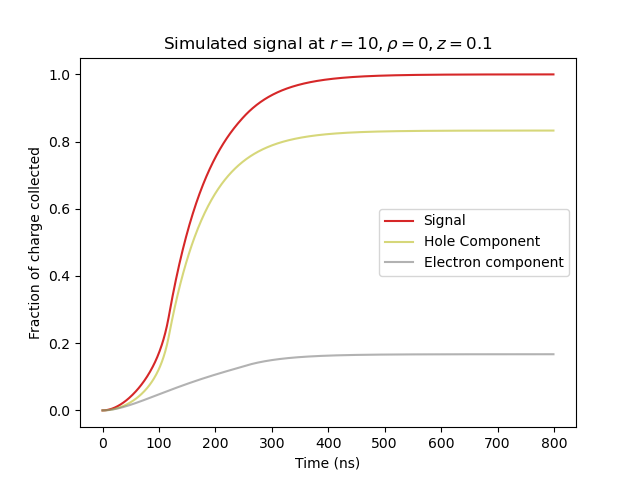
\includegraphics[width=0.49\linewidth]{ch3/figs/samp_wav_comp.png}
% \caption{A simulated event showing the path of holes and electrons and the corresponding waveform}.
% \label{fig:\texttt{siggen}_1d}
% \end{figure}

SolidStateDetectors.jl (\texttt{SSD}) is a software package developed by the group of Iris Abt at the Max Planck Institute Munich for the LEGEND experiment \cite{Abt:2021SSD}. It is written in Julia and can perform calculations in all 3 dimensions. \texttt{SSD} can calculate electric fields and potentials outside the detectors and has the ability for parallelization. The \texttt{SSD} enables full 3D diffusion and model self-repulsion in the signal. The charges are tracked individually using their position and velocity. The electic field calculation is done on GPUs. SSD provide a complete 3D simulation of the charges in Germanium along with surface drift, but the computational run time quickly scale with number of particles used. Alpha particles typically create a large charge cloud that would be difficult to model with current \texttt{SSD} version.

% In bulk, spherical charge cloud model works very well, but the charge cloud produced by alpha is not necessarily spherical due to the charge trapping and re-release effect on the passivated surface. A simulation to model alpha should allow for a nonspherical charge cloud while incorporating surface drift, diffusion, and self-repulsion.

% \begin{figure}
% \centering
% \includegraphics[width=0.49\linewidth]{ch3/figs/\texttt{SSD}_e.png}
% \includegraphics[width=0.49\linewidth]{ch3/figs/\texttt{SSD}_path.png}
% \caption{Simulated Electric field and charge paths in \texttt{SSD} simulations. It allows for calculations outside the detectors and in full 3 dimensions. \cite{\texttt{SSD}_web}.}
% \label{fig:\texttt{SSD}_plots}
% \end{figure}


\section{{\tdsim}}
{\tdsim} are new methods to simulate surface alpha events while directly simulating diffusion and self-repulsion effects. These are a dedicated model for surface interactions using 2-D approximations to optimize run time. They were initially programmed in C by David Radford and build upon \texttt{siggen}. As charges drift through the detectors, they keep track of charge densities at a pixel-by-pixel level, which allows for nonspherical charge clouds. The charges that end up on the surface have their velocities reduced by a predetermined factor. {\tdsim} also enables simulation of the effects of surface charges. The simulation is performed in r and z-direction while assuming $\phi$ symmetry—thus the charge cloud is simulated by a ring. Diffusion speed of 3D charge clouds. The charges that end up on the surface have their velocities reduced by a predetermined factor. {\tdsim} also enables simulation of the effects of surface charges.


Fig. \ref{fig:ehd_flowchart} shows how the {\tdsim} program works. The detector is divided into a grid, and charge densities are distributed at a given location based on the impact energy, usually over two adjacent grid points. The initial densities are determined using:

\begin{equation}
    \rho_H = \rho_E= \frac{\text{ E}\times 10^7 }{1000 \times 0.003 \times \text{grid}^3}
\end{equation}

where $\rho$ represents the charge pair density in units of \(10^{10}/\text{cm}^3\). The deposited energy E is the deposited energy in keV, which is first converted to MeV by dividing by 1000.0. The factor of \(10^7\) is to get final unit correct. The denominator includes \(0.003\), which represents the approximate energy required to generate an electron-hole pair in Germanium. Finally, dividing by \(\text{grid}^3\) normalizes the number of generated charge pairs to the grid volume. The density for both holes and electrons are deposited equally in points (z,r) and (z+1,r).

The boundary conditions are set according to the detector geometry, impurity concentration, surface charge, and bias voltage. Then electric potential and weighting potential are calculated using an over-relaxation algorithm. The capacitance and depletion are estimated. Undepleted regions of a semiconductor detector have no net space charge and no electric field and are indicated by a local minimum in the electrical potential. The capacitance is calculated by relating two equations for the energy stored in a capacitor.

\begin{equation}\label{capacitance_eq}
C= \frac{\epsilon}{V^2} \int_{}^{} E^2 dA
\end{equation}

\begin{figure}[!htb]
\centering
%[trim={left bottom right top},clip]
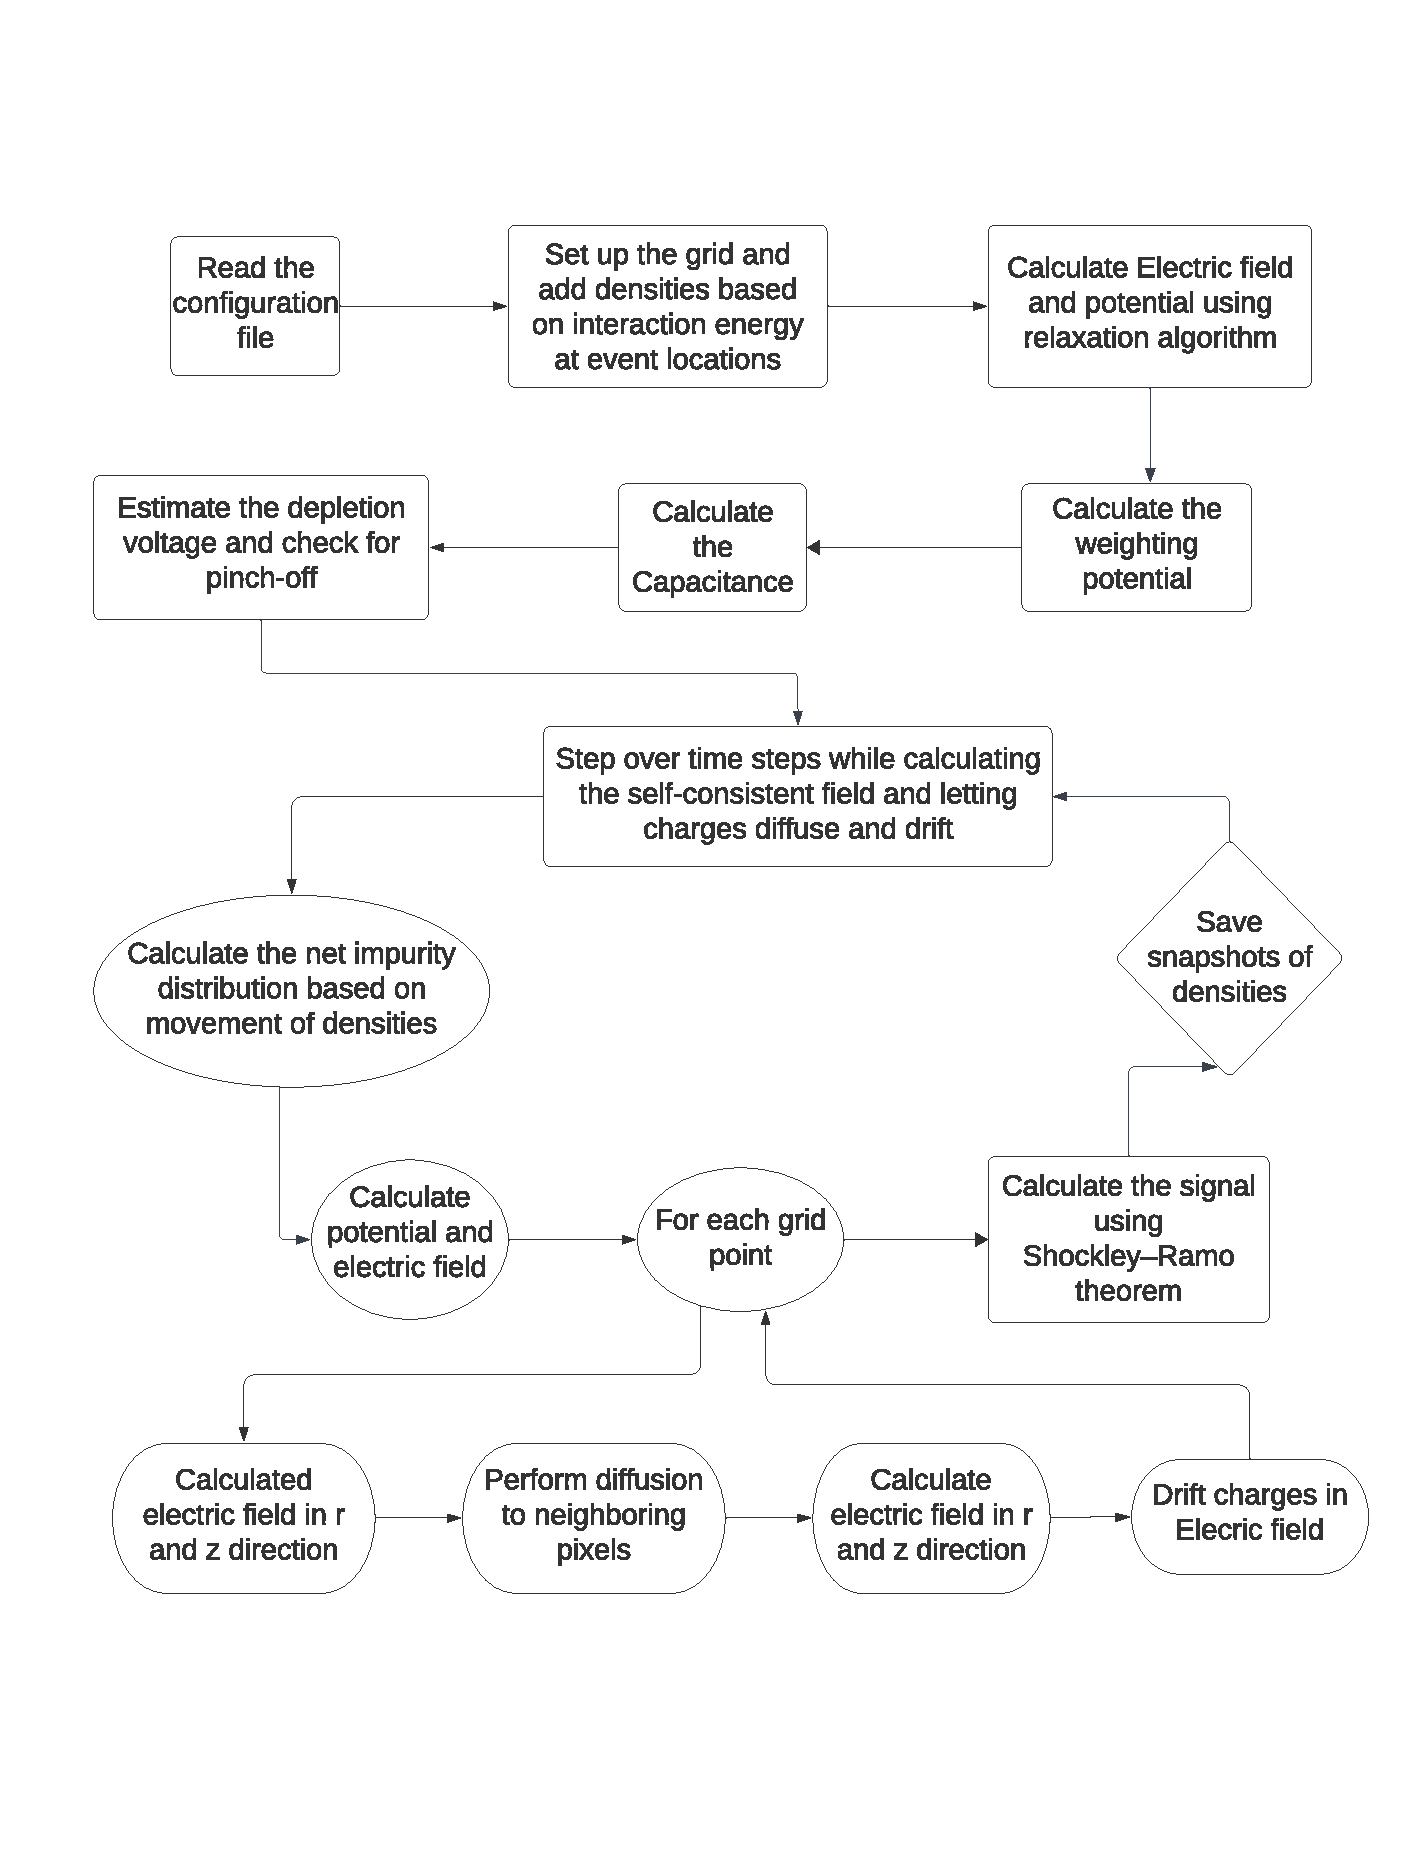
\includegraphics[width=0.99\linewidth,trim={2pc 10pc 1.5pc 9pc},clip]{ch3/figs/ehd_flowchart.pdf}
\caption{A flow chat illustration the pseudo code for {\tdsim}.}
\label{fig:ehd_flowchart}
\end{figure}


After the initial setup, the program steps through a small time step. The charges are allowed to diffuse and then drift in the electric field. The net impurity distribution is updated based on the movement of these charges using:


\section{Diffusion}
Diffusion arises from random thermal motion of electrons and holes, causing them to spread out from regions of high concentration into regions of lower concentration. In thermal equilibrium, the diffusion coefficient $D$ and the mobility $\mu$
are related by the Einstein relation:
\begin{equation}
D = \mu \frac{k_B T}{q},
\end{equation}
where $k_B$ is Boltzmann's constant, $T$ is the absolute temperature, and $q$ is
the elementary charge. Thus, if the mobility $\mu$ is known or has been fit to
experimental data, $D$ may be determined for a specified temperature. In
germanium at cryogenic temperatures (e.g., $\sim 77$\,K), the mobilities are
sufficiently large that diffusion can still have a noticeable effect on the
final spread of a charge cloud, although it is smaller compared to room
temperature conditions.


Carrier diffusion in the simulation is handled by redistributing charge among
neighboring grid cells in both the radial $(r)$ and axial $(z)$ directions.
During each time step $\Delta t$, a fraction of the carriers in cell $(z,r)$
diffuse to the adjacent cells $(z\pm1,\,r\pm1)$ according to two quantities: $\delta_z$ and $\delta_r$

These fractions are computed from an approximate diffusion parameter 
$f$ and the local drift velocity magnitudes $\lvert \mathbf{v_z} \rvert$, 
$\lvert \mathbf{v_r} \rvert$ as follows:
\begin{align}
   \delta_z &\;=\; \frac{\Delta x \;\,v_z \;f}{E_z}\label{eq:deltaez}\\
   \delta_r &\;=\; \frac{\Delta x \;\,v_r \;f}{E_r} \label{eq:deltaer}
\end{align}
where $\Delta x$ is the grid size, 
$v_{z}$ and $v_{r}$ are the drift velocities, 
$E_{z}$ and $E_{r}$ are the local field components, 
and $f$ incorporates the diffusion coefficient $D$ and corrections for grid sizes.
If $E_z$ or $E_r$ is below $1\,\mathrm{V/cm}$, the code sets 
$\delta_z = 0$ or $\delta_r=0$ under the assumption that low-field regions produce negligible drift velocity.


\subsection{Volume Correction}

In cylindrical $(r,z)$ coordinates, each radial ring has a different 
physical area. The simulation tracks these scaling factors with arrays 
\(\texttt{s1}[r]\) and \(\texttt{s2}[r]\). In essence,
\[
\texttt{s1}[r] \;\approx\; 1 + \frac{0.5}{r-1}, 
\qquad
\texttt{s2}[r] \;\approx\; 1 - \frac{0.5}{r-1},
\] 
(plus special handling at $r=1$). These scalars adjust how much 
charge diffuses into or out of the neighboring ring to ensure charge conservation in cylindrical geometry. Specifically, 
if $\delta_r$ is the fraction of carriers leaving cell $(r)$ in 
the $+r$ direction, the actual increment in the neighbor cell 
$(r+1)$ is multiplied by $\texttt{s1}[r]$, while the old cell is 
reduced by the same fraction multiplied by $\texttt{s1}[r]$ to 
balance volume differences. Similarly, diffusion to cell $(r-1)$ 
uses $\texttt{s2}[r]$.

\section{Charge Update}

This approach enforces that if $r$ changes by one grid index, 
the annular circumference changes from $2\pi (r-1)$ to $2\pi r$, 
or $2\pi (r-2)$ in the negative direction. Hence, we apply factors
\(\texttt{s1}\) and \(\texttt{s2}\) to rescale the transferred 
charge, ensuring the total density remains physically consistent.

After computing the diffusion fractions $\delta_z$ and $\delta_r$, 
the code subtracts those amounts from the central cell's carrier density 
and adds them to the four neighbors:
\begin{align}
  \rho^{\mathrm{new}}(z,\,r+1) &\;\mathrel{+}= \;\rho^{\mathrm{old}}(z,\,r)\times\delta_r \times s_1(r) \times \frac{r-1}{r} \label{ch3:eq:diffusion_update_1} \\
  \rho^{\mathrm{new}}(z-1,\,r) &\;\mathrel{+}= \;\rho^{\mathrm{old}}(z,\,r)\times\delta_z \label{ch3:eq:diffusion_update_2} \\
  \rho^{\mathrm{new}}(z+1,\,r) &\;\mathrel{+}= \;\rho^{\mathrm{old}}(z,\,r)\times\delta_z \label{ch3:eq:diffusion_update_3} \\
  \rho^{\mathrm{new}}(z,\,r-1) &\;\mathrel{+}= \;\rho^{\mathrm{old}}(z,\,r) \times \delta_r \times s_2(r) \times\frac{r-1}{r-2} \label{ch3:eq:diffusion_update_4}.
\end{align}
 
Because the radially adjacent cells differ in annular circumference, 
multiplying by \(\texttt{s1}[r]\) or \(\texttt{s2}[r]\) 
helps maintain overall normalization.

\section{Drift in Electric Field}

During the charge drift we calculate the electric field in r and z direction at each gird point. We then use a piecewise linear interpolation to compute the drift velocity $v(E)$ from the local electric field $E$. We define an array of electric field breakpoints, $\texttt{drift\_E}[]$, which partition the field
range into intervals. For each interval $[E_i, E_{i+1}]$, we store two quantities: a drift offset, corresponding to the drift velocity at $E = E_i$, and a drift slope which is the rate of change of drift velocity with respect to the electric field in that interval. The drift velocity is then
computed by:
\[
v(E) \;=\; \text{drift offset}[i]
\;+\; \text{drift slope}[i] \,\bigl( E - E_i \bigr),
\]
with $E_i \le E < E_{i+1}$. The fig. \ref{ch3:fig:dv_vs_e} shows the relation for the Drift Velocity verses Electric field. The dirft velocity is then multiplied by the time step to find where the charges will drift and then the charges are moved to new location.

\begin{figure}
    %[trim={left bottom right top},clip]
    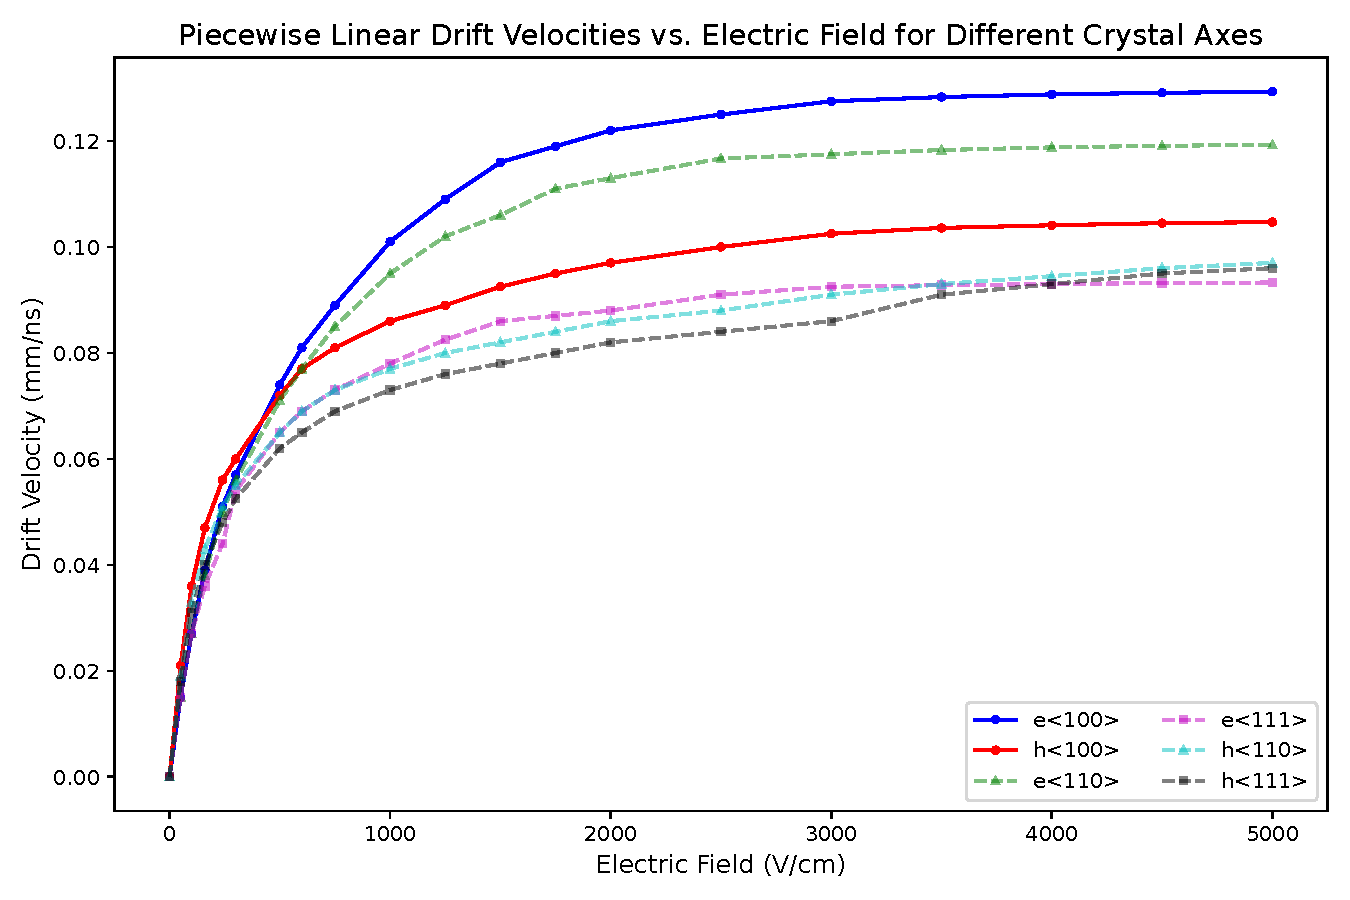
\includegraphics[trim={0cm 0 0cm 0},clip,width=0.99\linewidth]{ch3/figs/ehd_dv_e.pdf}
    \caption{Relation of drift velocity verses electric field in {\tdsim}. Only 100 direction velocities are used in the current model.}
    \label{ch3:fig:dv_vs_e}
\end{figure}

\subsection{Fraction Splitting}\label{ch3:sec:frac_split}

To conserve charge when drifting carriers from one grid cell to another,
we use a splitting approach. Suppose
that after a time step $\Delta t$, the carrier density in grid cell $(z,r)$
moves to a new position with integer indices $(k,i)$ plus fractional parts
$f_z$ and $f_r$:
%
\[
k \;=\; z + \lfloor \Delta z \rfloor,\quad
f_z \;=\; \Delta z - \lfloor \Delta z \rfloor,
\]
(and similarly for the radial indices). Thus,
\begin{align}
&\text{fraction in }(k, i)   \;=\; f_{r} \times f_{z} \\
&\text{fraction in }(k, i+1) \;=\; (1 - f_{r}) \times f_{z}\\
&\text{fraction in }(k+1, i) \;=\; f_{r} \times (1 - f_{z})\\
&\text{fraction in }(k+1, i+1)\;=\; (1 - f_{r}) \times (1 - f_{z}).
\label{eq:bilinear-fractions}
\end{align}

Hence, if $\rho^{\mathrm{old}}(z,r)$ is the charge density in the old cell,
the new distribution is updated by
\begin{align}
\rho^{\mathrm{new}}(k,i)   &\,\mathrel{+}=\, \rho^{\mathrm{old}}(z,r)\times \bigl[f_{r}\,f_{z}\bigr] \times \text{G}_{r,z} \label{ch3:eq:den_update_1} \\
\rho^{\mathrm{new}}(k,i+1) &\,\mathrel{+}=\, \rho^{\mathrm{old}}(z,r)\times \bigl[(1 - f_{r})\,f_{z}\bigr] \times \text{H}_{r,z} \label{ch3:eq:den_update_2} \\
\rho^{\mathrm{new}}(k+1,i) &\,\mathrel{+}=\, \rho^{\mathrm{old}}(z,r)\times \bigl[f_{r}\,(1 - f_{z})\bigr] \times \text{G}_{r,z} \label{ch3:eq:den_update_3} \\
\rho^{\mathrm{new}}(k+1,i+1)&\,\mathrel{+}=\, \rho^{\mathrm{old}}(z,r)\times \bigl[(1 - f_{r})\,(1 - f_{z})\bigr] \times \text{H}_{r,z}. \label{ch3:eq:den_update_4}
\end{align}
\subsection{Geometric Factors}
\label{sec:geom-factor}

In cylindrical coordinates, each cell at index $r$ corresponds to an annular
region of approximate circumference $2\pi (r \,\Delta r)$ and thickness
$\Delta z$. When charge moves from cell $(z,r)$ to cell $(k,i)$, we
often apply the factors:

\[
\text{G}_{r,z} \;\equiv\; \frac{(r-1)}{(i-1)}
\qquad
\text{H}_{r,z} \;\equiv\; \frac{(r-1)}{(i)}
\] 


reflecting the difference in annular volumes at radii $r$ and $i$.
The offsets $(r-1)$ and $(i-1)$ arise from one-based indexing in the code. By multiplying the bilinear fractions by $\Gamma_{r,z}$, the simulation conserves total charge when rings expand or contract in radius.In practice, near $r=0$ or $i=0$, the geometric factor $\Gamma_{r,z} \;=\; (r-1)/(i-1)$ would be undefined or negative. Hence, the actual code checks whether $r$ or $i$ is zero or one, and uses a modified factor that preserves volume scaling. 

% The factors \verb|8*r - 8| or \verb|8*i - 8| are specialized scalings to approximate the annular volume near the central axis or near $i=0$. They ensure that even when $r$ or $i$ equals 0 or 1, the total charge remains consistent with the expected geometry. For example, at the very center ($r=0$), a full ring circumference does not exist, so a smaller effective volume must be used. Although such \verb|8*-8| scalings can appear ad~hoc, they are designed to smoothly transition from the central axis to the first few radial rings, thereby avoiding division by zero while preserving charge.

\section{Surface Drift}

When charge carriers drift within the detector, they may encounter passivated surfaces, which require special handling due to their impact on charge collection. If this new position falls within a passivated surface region, the charge interaction with the surface must be accounted for. To model the surface, the lowest grid point is divided into length of surface and grid-surface. We store the charges on surface in a special row. 

If the charge drifts completely into the surface, it is fully added to the surface row. If the charge enters the passivated layer, we split it up using the fraction splitting described in \ref{ch3:sec:frac_split}. Similarly charges from the surface can drift to the bulk and other surface points. While performing the diffusion on the last grid point in \ref{ch3:eq:diffusion_update_2}, the bottom z point is considered the surface. Similarly any point on the surface can diffuse up or to other points on the surface. The drift and rate of diffusion on the surface is suppressed by the surface-drift-velocity factor. This factor is typical about 0.001 is the ratio of the speed on the surface to the bulk. This helps model the slow rising tail of the surface backgrounds.


\section{Impurity Correction}
Surface events create large amount of charge carries that could impact local impurity and must be corrected to accurately calculate the electric potential. At a given time impurity corrections is given by:

\begin{equation}
  {\text{Impurity}_{t}}(z, r) = \text{Impurity}_{0}(z, r) +
  \bigl( \rho_h(z, r) - \rho_e(z, r) \bigr) \times \frac{e}{\epsilon} \times \frac{(\Delta x)^2}{2}.
\end{equation}
The $\text{Impurity}_{0}$ is the impurity of the crystal from production. $\rho_h(z,r)$ and $\rho_e(z,r)$ are the hole and electron densities respectively. $\frac{e}{\epsilon}$ is the conversion factor that relates charge density to the resulting electric field, derived from Gauss’s law in Germanium with $\epsilon = 16\epsilon_0$. $\frac{e}{\epsilon} = 11.310$ in 
charge units $10^{10}\frac{e}{cm^3}$. $(\Delta x)^2$ is the area of the grid which converts density into charge and then the conversion factor converts it into $10^{10}\frac{e}{cm^3}$ units to match the units of impurity used.

\section{Signal Calculation}
In cylindrical coordinates, each grid cell at radius $r$ and height $z$ has an approximate area proportional to $(r - 1)$. Once we read the electron 
density $\rho_e(r,z)$ and hole density $\rho_h(r,z)$ at time $t$, the weighted sums are defined as:
\begin{align}
S_e(t) \;=\; \sum_{z=1}^{L-1} \sum_{r=1}^{R-1}
   \rho_e(r,z)\,\bigl(r-1\bigr)\,\text{wpot}[r-1][z-1],\\
S_h(t) \;=\; \sum_{z=1}^{L-1} \sum_{r=1}^{R-1}
   \rho_h(r,z)\,\bigl(r-1\bigr)\,\text{wpot}[r-1][z-1],
\end{align}
where \(\texttt{wpot}[\,r-1\,][\,z-1\,]\) is the weighting potential at that grid 
point. These $S_e(t)$ and $S_h(t)$ represent the induced signal contributions 
from electrons and holes respectively via Shockley Ramo’s theorem.

The initial unweighted sums are defined as:
\begin{align}
R_{e}(0) \;=\; \sum_{z=1}^{L-1} \sum_{r=1}^{R-1}
   \rho_e(r,z)\,\bigl(r-1\bigr), \quad \\
R_{h}(0) \;=\; \sum_{z=1}^{L-1} \sum_{r=1}^{R-1}
   \rho_h(r,z)\,\bigl(r-1\bigr), \quad
\end{align}
% They keep track of how many electrons or holes remain in the crystal at time $t$ 
% (as opposed to how much they contribute to the signal).  For instance, if 
% $R_{h}(t)$ drops below $R_{h}(0)$, that implies some fraction of holes 
% has reached the collecting electrode or left the active region.

Combining these quantities, the net induced signal can be computed as
\begin{equation}
\text{Signal}[\,t\,] 
\;=\;
  \frac{\,S_h(t)\;-\;S_h(0)\,}{\,R_{h}(0)\,}
  \;-\;
  \frac{\,S_e(t)\;-\;S_e(0)\,}{\,R_{e}(0)\,}
\label{eq:net-signal}
\end{equation}
By subtracting the electrons’ contribution 
(negative) from the holes’ (positive), this formula matches the typical polarity 
where holes drift toward the readout electrode and electrons may drift in the 
opposite direction. Normalizing by $R_{e}(0)$ and $R_{h}(0)$ ensures that the 
signal is expressed as a fraction of the original total electron/hole count, 
so it starts near zero at $t=0$ and approaches some final value as all charges 
arrive at the contacts.



\section{Density Snapshots}
\begin{figure}[!htb]
    %[trim={left bottom right top},clip]
    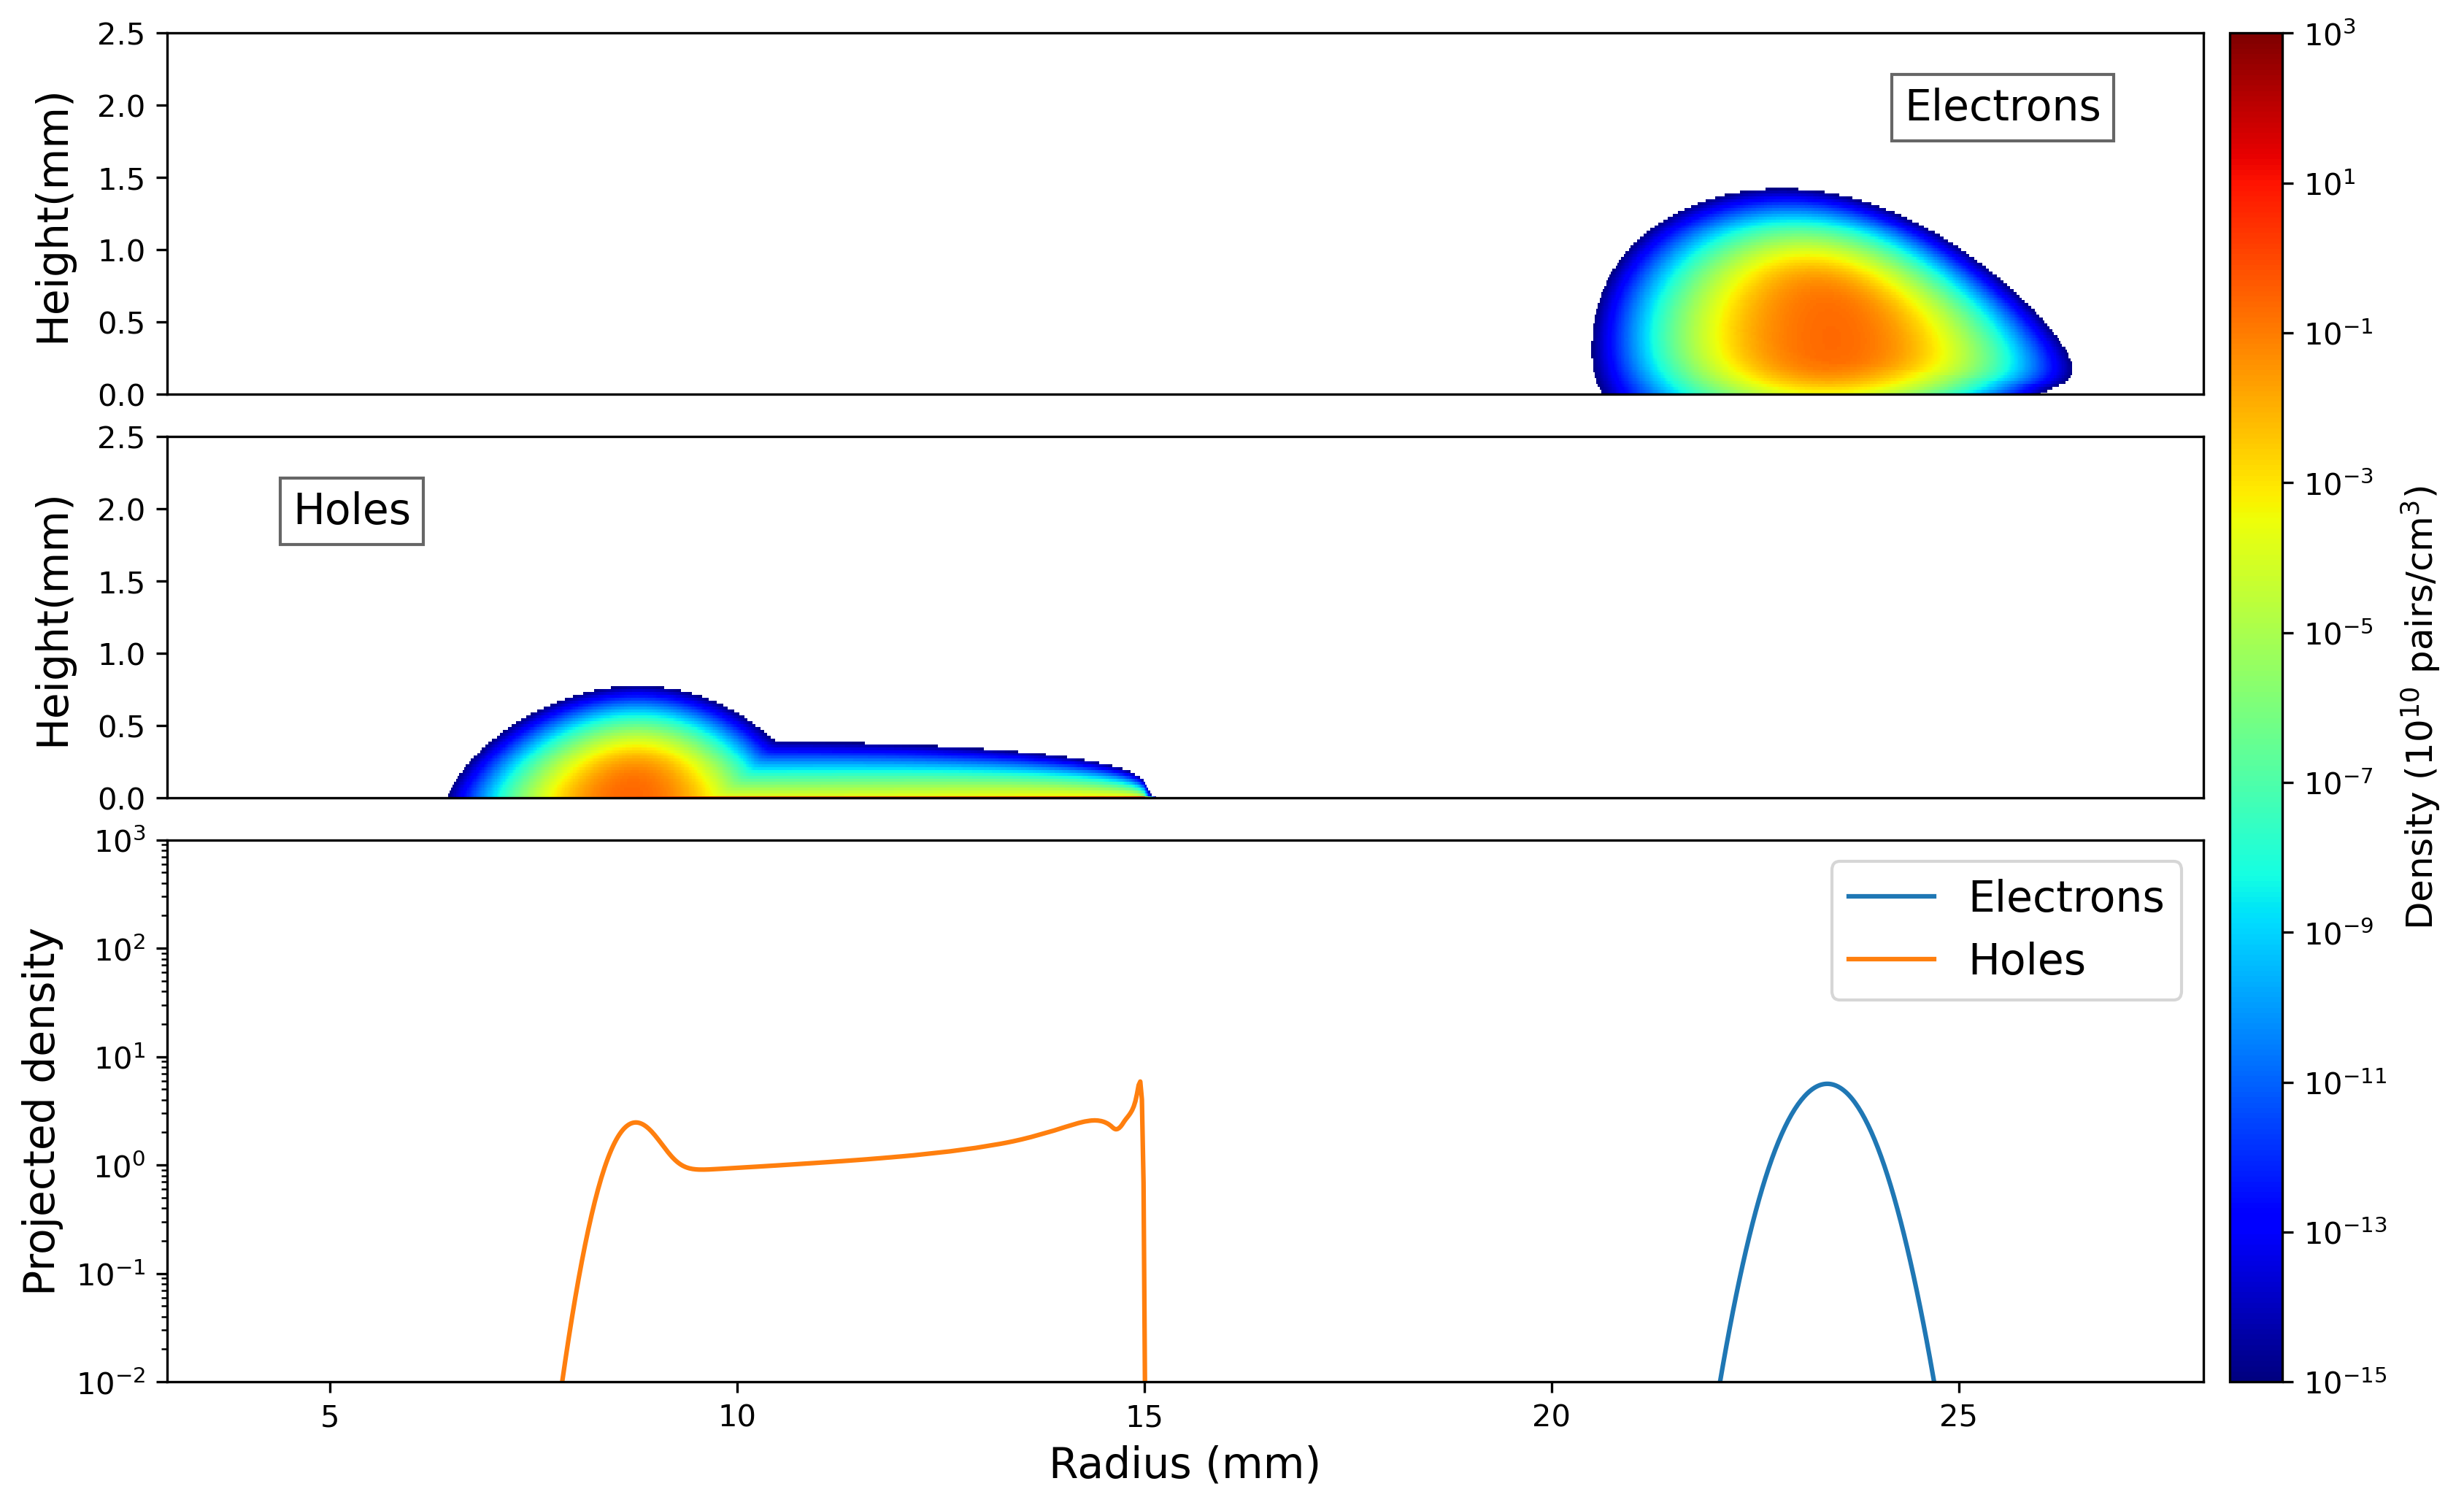
\includegraphics[trim={0cm 0 0cm 0},clip,width=0.99\linewidth]{ch3/figs/drift_path_sc=-0.3.png}
    \caption{Drift of electron and hole charge clouds in {\tdsim}. The negative surface charge pulls the holes onto the surface which move at a slower speed.}
    \label{ch3:fig:ehd_path_pd_sc-0.3}
\end{figure}

\begin{figure}[!htb]
    %[trim={left bottom right top},clip]
    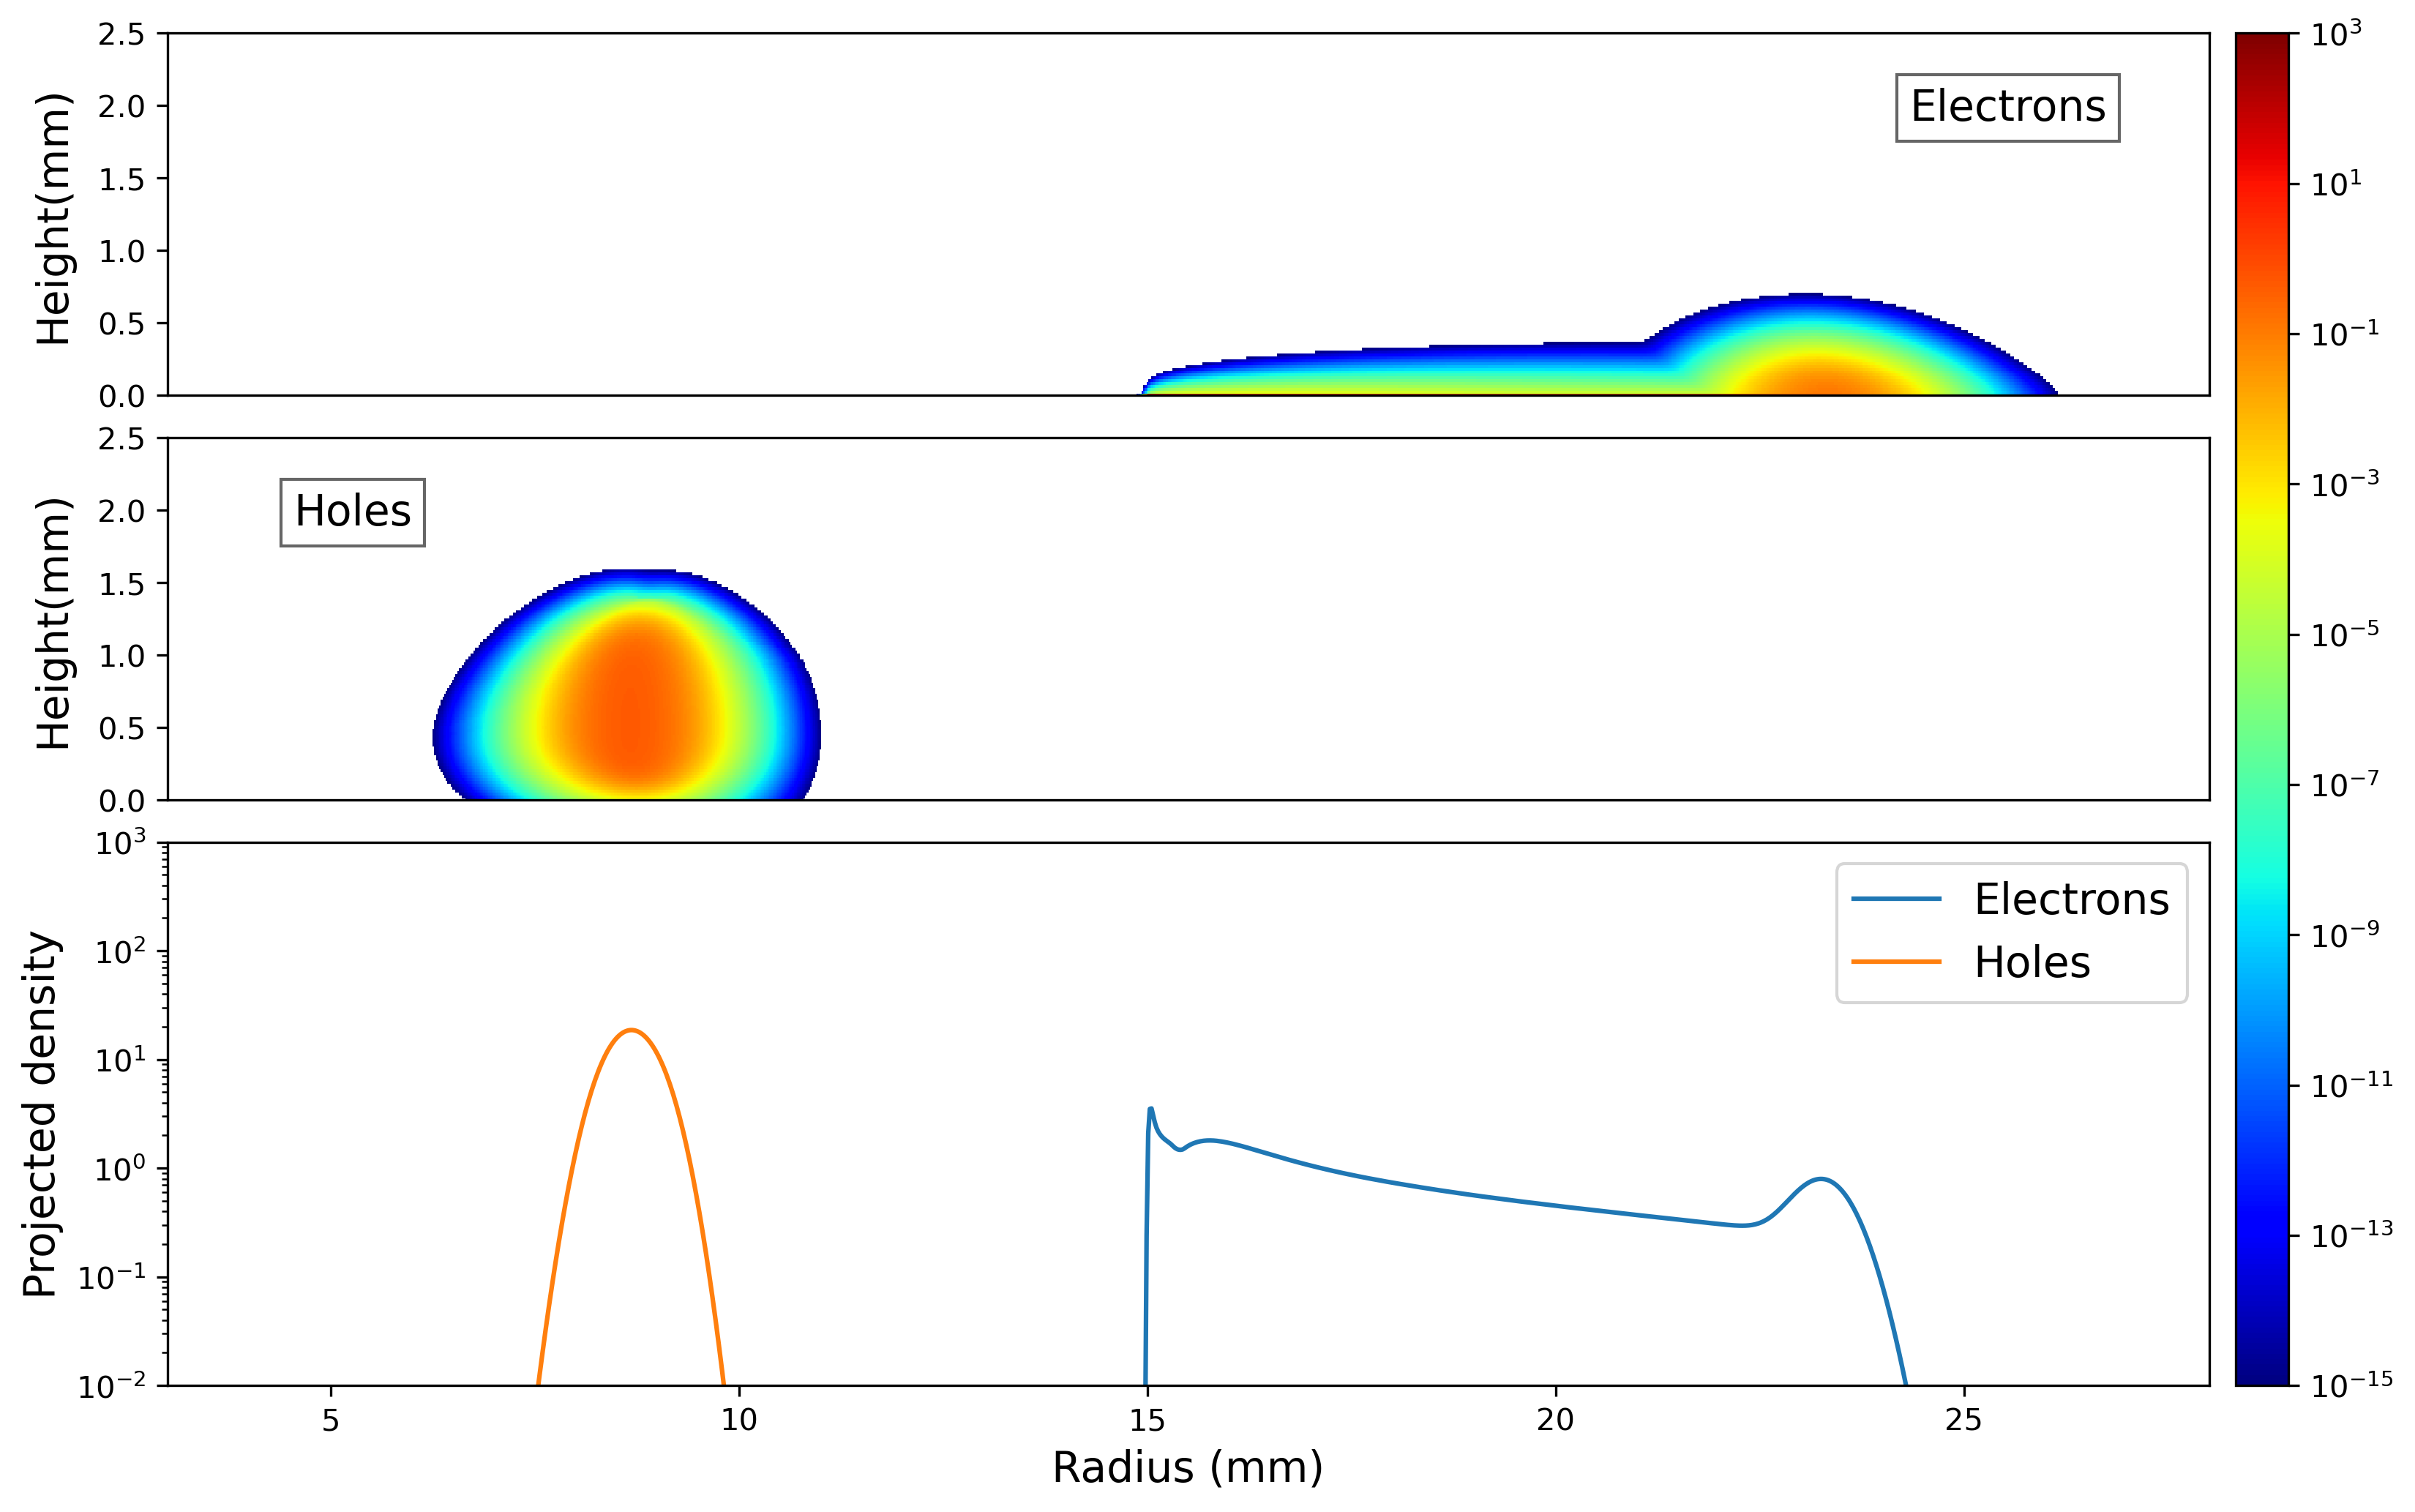
\includegraphics[trim={0cm 0 0cm 0},clip,width=0.99\linewidth]{ch3/figs/drift_path_sc=0.3.png}
    \caption{Drift of electron and hole charge clouds in {\tdsim}. The positive surface charge pulls the electrons onto the surface which move at a slower speed.}
    \label{ch3:fig:ehd_path_pd_sc0.3}
\end{figure}

\begin{table}[!htb]
    \centering
    \renewcommand{\arraystretch}{1.3} % Adjust row spacing
    \begin{tabular}{|l|p{10cm}|c|}
        \hline
        \textbf{Flag} & \textbf{Description} & \textbf{Example} \\ 
        \hline
        -r & Set the radial position of the event in mm. & 15.00 \\
        \hline
        -z & Set the axial position of the event in mm. & 0.50 \\
        \hline
        -g & Specify the detector name. & P42575A \\
        \hline
        -s & Set the surface charge density in $10^{10} e/\text{cm}^2$. & -0.50 \\
        \hline
        -e & Input the interaction energy in keV. & 5000 \\
        \hline
        -v & Choose whether to write density files (0 = no, 1 = yes). & 1 \\
        \hline
        -f & Choose whether to recalculate the electric field (0 = no, 1 = yes). & 1 \\
        \hline
        -w & Choose whether to save the electric field (0 = no, 1 = yes). & 1 \\
        \hline
        -d & Choose whether to save the depletion surface (0 = no, 1 = yes). & 1 \\
        \hline
        -p & Choose whether to write the weighting potential (0 = no, 1 = yes). & 1 \\
        \hline
        -b & Set the bias voltage in volts. & 3500 \\
        \hline
        -h & Specify the grid size in mm. & 0.0200 \\
        \hline
        -m & Define the passivated surface depth in mm. & 0.10 \\
        \hline
        -c & Set the velocity of surface charges compared to bulk. & 0.75 \\
        \hline
        -a & Input a custom impurity density profile file. & filename.dat \\
        \hline
        -t & Define the total simulation run time in ns. & 16000 \\
        \hline
        -u & Set the frequency of output signal saving in ns. & 16 \\
        \hline
    \end{tabular}
    \caption{Input parameters to EH-Drift}
    \label{tab:ehdrift_parameters}
\end{table}

\begin{figure}[!htb]
    %[trim={left bottom right top},clip]
    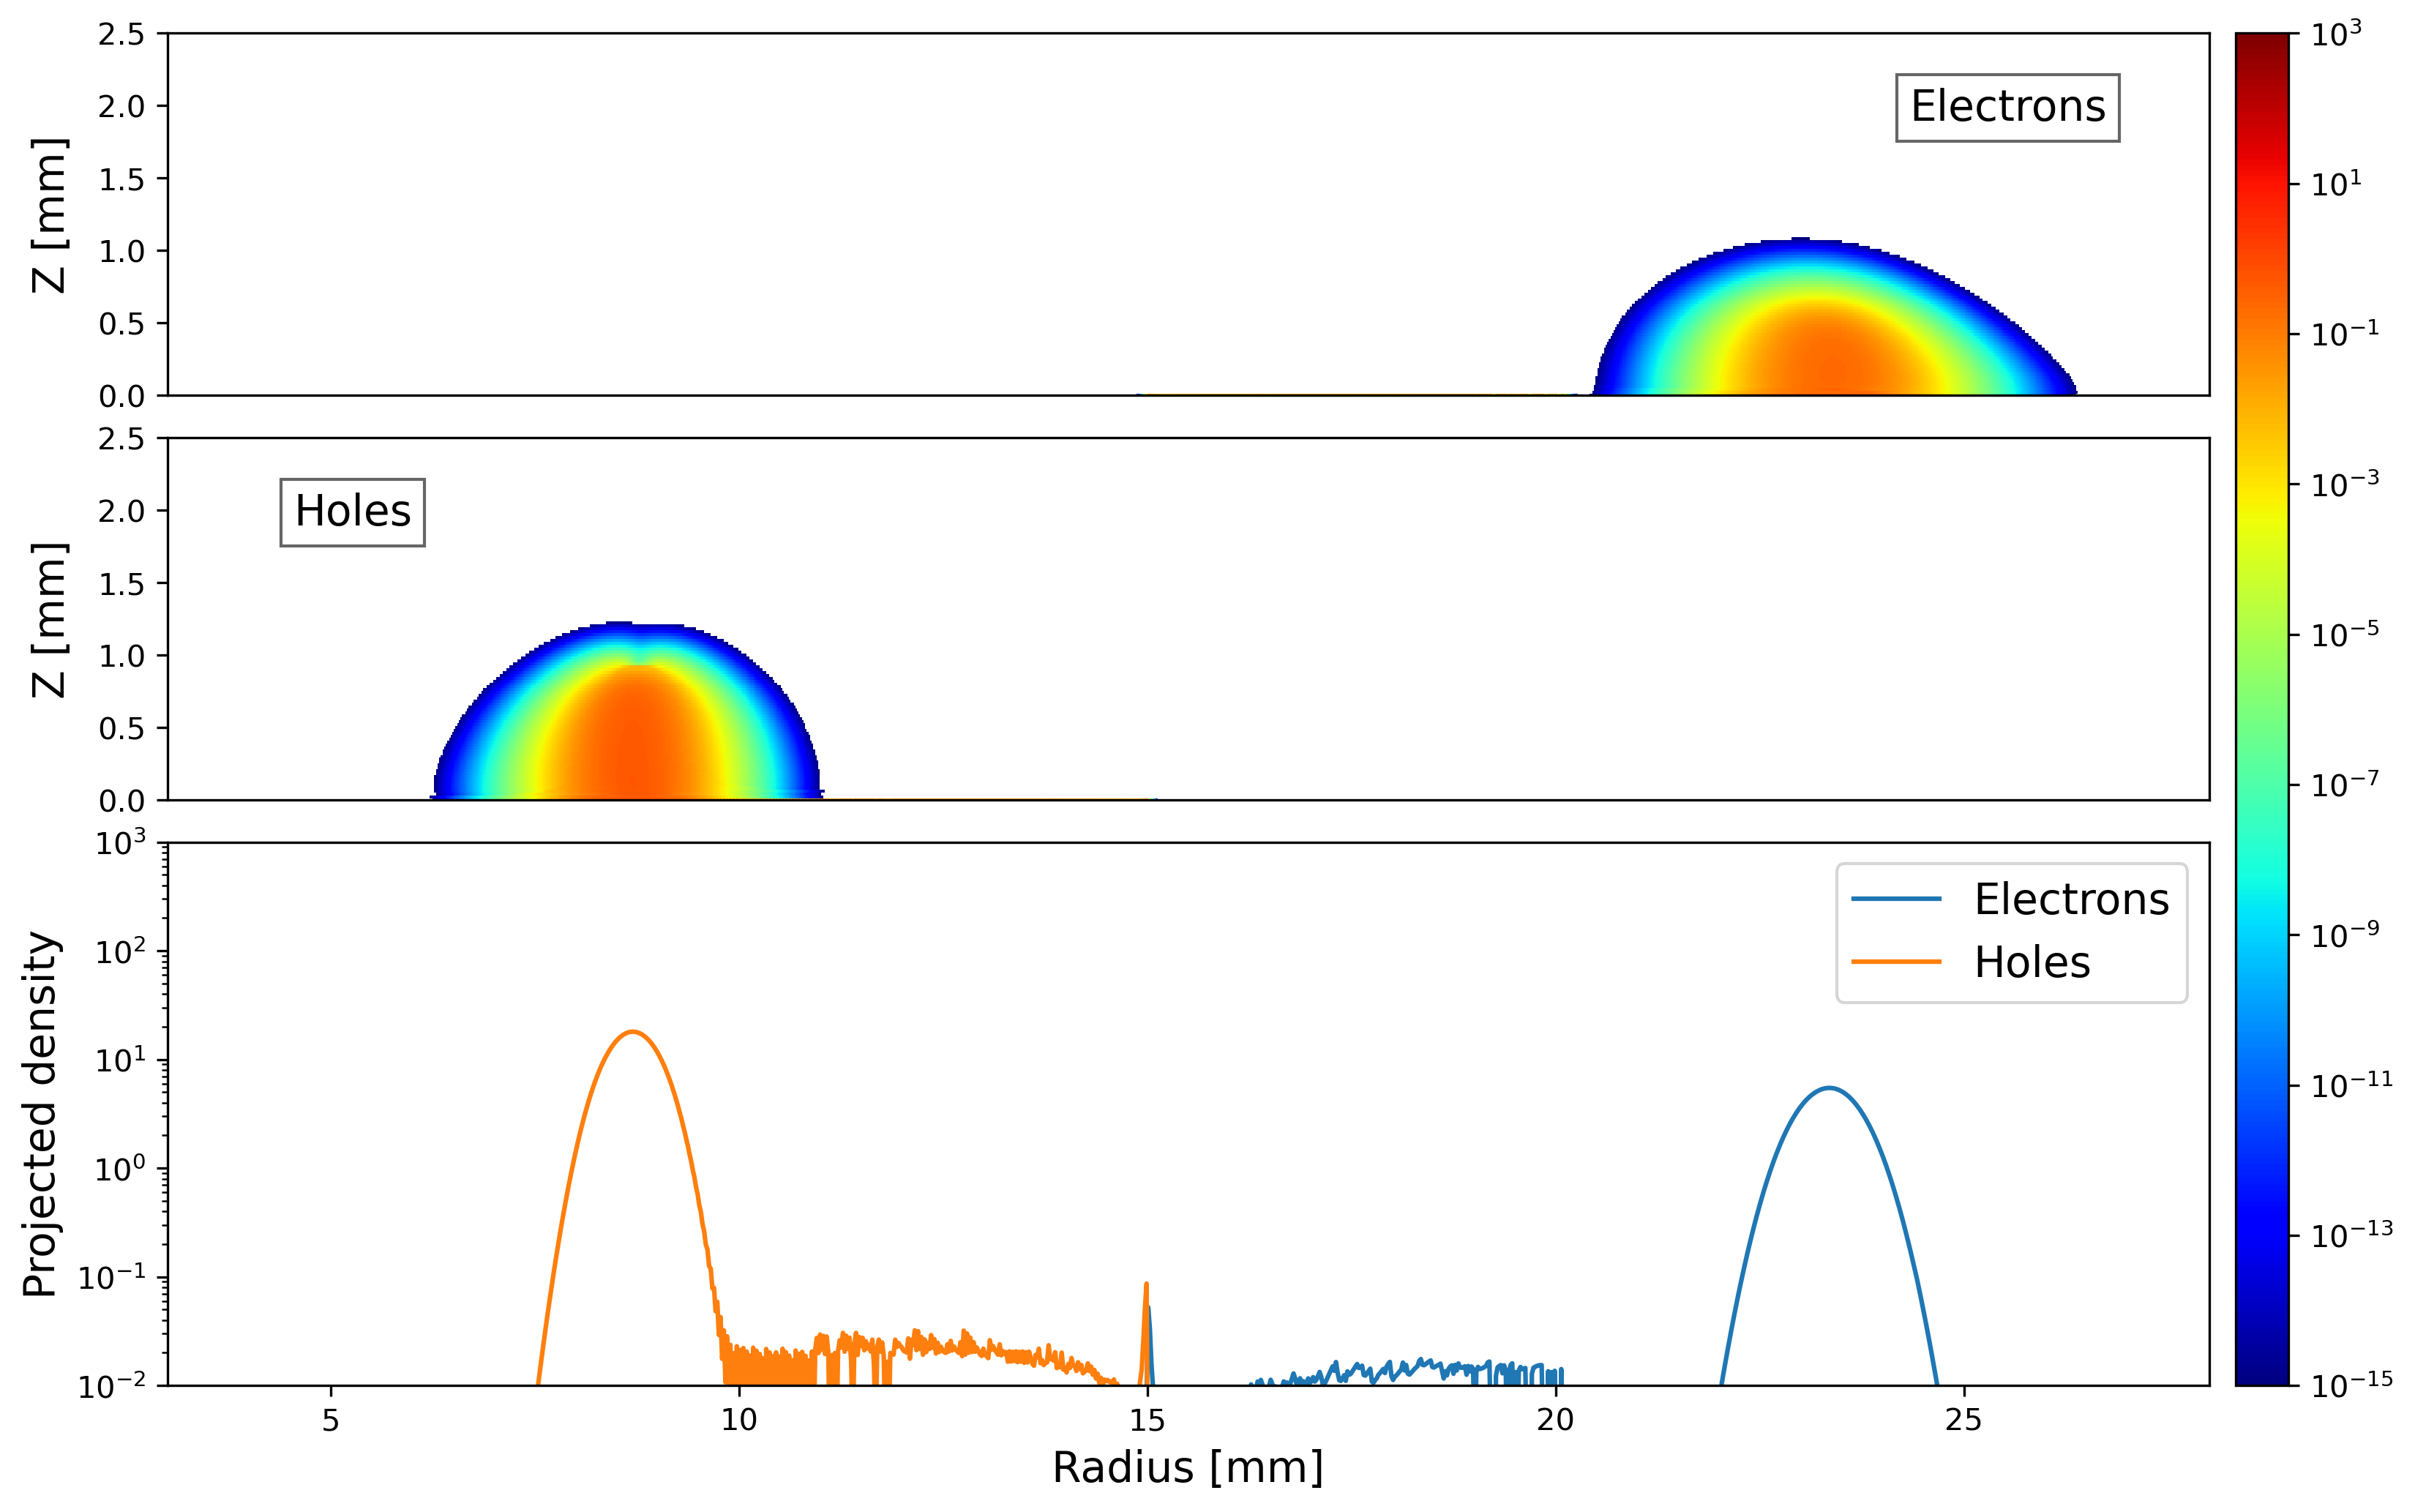
\includegraphics[trim={0cm 0 0cm 0},clip,width=0.99\linewidth]{ch3/figs/drift_path_sc=0.0.png}
    \caption{Drift of electron and hole charge clouds in {\tdsim}. The projected densities show how the charges are distribution along the radius. The density have two peak, one due to fast moving component in bulk and another due to slow moving component on the surface.}
    \label{ch3:fig:ehd_path_pd_sc0}
\end{figure}



Fig. \ref{ch3:fig:ehd_path_pd_sc0} shows a snapshot at time=$80$ns of the electron and hole clouds drift in the {\tdsim} for a 5 MeV energy deposition close to the surface with no charge. The projected density shows the distribution of the charge in the cloud. The head of each signal has a peak which is where charges would have normally traveled in point charge simulations. The tail of the projected density has a peak that is due to the slow drift of the charges on the surface. The drift on the surface, in this case, is set to be $1000$ slower than drift in bulk. This matches the range of possible effects found in \cite{MULLOWNEY201233}. 

{\tdsim} also provides several custom tunable parameters such surface charge, surface to bulk drift ration, initial energy, etc. that can be used to match the data. Fig. \ref{fig:wf_comp} shows how the output changed with surface to bulk drift and surface charge. High surface charge means that more charges will be pulled onto the surface and thus less sharp rising part will have lower magnitude. A faster surface to bulk ration means that the charges on the surface will be collected fast and so the tail shape will be different.

\begin{figure}[!htb]
    %[trim={left bottom right top},clip]
    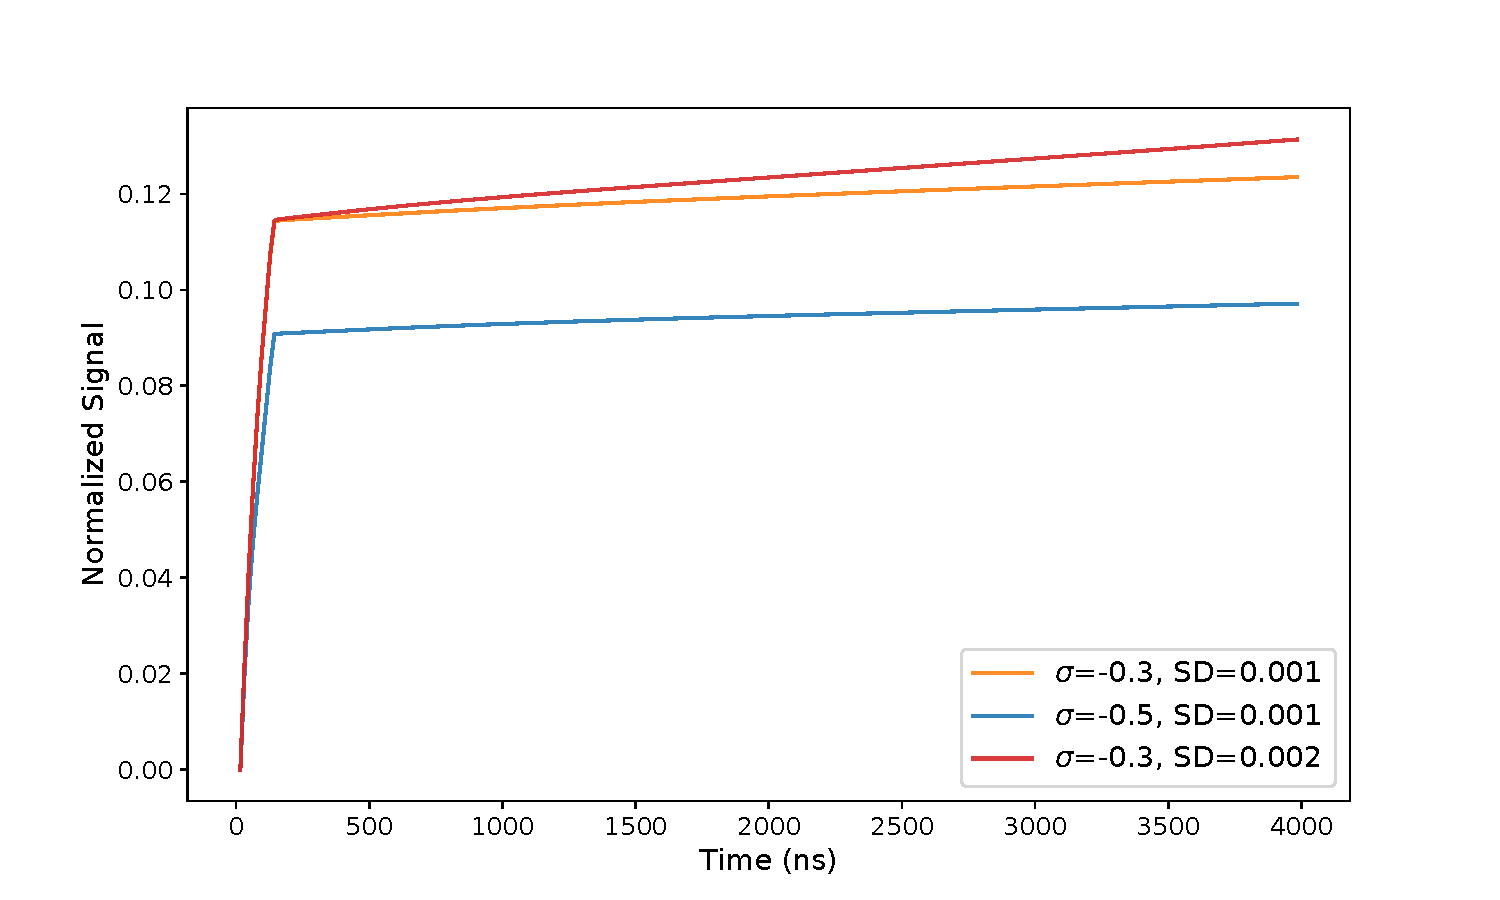
\includegraphics[trim={0.1cm 0.3cm 1.3cm 0.3cm},clip,width=0.99\linewidth]{ch3/figs/wf_comp.pdf}
    \caption{A comparison of waveforms generated by {\tdsim} for a {\Ltwo} PPC detector based of different tunable parameters surface charge ($\sigma$) and relative surface drift velocity (SD).}
    \label{fig:wf_comp}
\end{figure}



\section{Input and Output}

The simulation output is stored in an HDF5 file, a hierarchical data format optimized for handling large structured datasets. Each simulated event is recorded in the "event data" dataset as a compound data type containing energy, radius and height positions, surface charge, and surface drift velocity factor and the signal for the event. The dataset is dynamically extendable, allowing new events to be appended without rewriting existing data. The file includes grid size, passivated surface thickness, self-repulsion flag, and detector name as attributes. Attributes are stored as scalars at the file root level for efficient retrieval without redundancy. This storage is critical for High Performance Computing (HPC) when we simulate thousands of waveforms for multiple detectors.
 